\documentclass[a4paper,fleqn]{cas-sc}

\usepackage[numbers,sort&compress]{natbib}
\usepackage{amsmath,amssymb}
\usepackage{booktabs}
\usepackage{multirow}
\usepackage{graphicx}
\usepackage{xurl}
\usepackage{microtype}
\usepackage{siunitx}
\usepackage{placeins}
\usepackage{soul}
\sethlcolor{yellow}

\begin{document}
\let\WriteBookmarks\relax
\def\floatpagepagefraction{0.9}
\def\textpagefraction{0.05}

\shorttitle{Insulin dose--response in type 1 diabetes}
\shortauthors{J.C. Wolber}

\title[mode=title]{\hl{Insulin Dose--Response Alignment for Glucose Forecasting}\\
\hl{in Type~1 Diabetes}}

\author[1,2]{Jonas C. Wolber}
\cormark[1]
\ead{jwolber@ukaachen.de}
\credit{Conceptualization, Methodology, Software, Validation, Formal analysis,
Writing -- original draft, Writing -- review and editing}

\author[2]{Moein E. Samadi}
\ead{mesamadi@ukaachen.de}
\credit{Conceptualization, Methodology, Writing -- review and editing}

\author[1, 3]{Julia Sellin}
\ead{jsellin@ukaachen.de}
\credit{Project administration, Writing -- review and editing}

\author[1, 3]{Martin Mücke}
\ead{mamuecke@ukaachen.de}
\credit{Project administration, Writing -- review and editing}

\author[2]{Andreas Schuppert}
\ead{aschuppert@ukaachen.de}
\credit{Supervision, Project administration, Writing -- review and editing}

\affiliation[1]{organization={Institute for Digital General Practice},
                addressline={University Hospital RWTH Aachen, Pauwelsstra{\ss}e 30},
                city={Aachen},
                postcode={52074},
                country={Germany}}
\affiliation[2]{organization={Institute for Computational Biomedicine},
                addressline={RWTH Aachen University, Pauwelsstra{\ss}e 30},
                city={Aachen},
                postcode={52074},
                country={Germany}}
\affiliation[3]{organization={Center for Rare Diseases},
addressline={RWTH Aachen University, Pauwelsstra{\ss}e 30},
city={Aachen},
postcode={52074},
country={Germany}}
\cortext[1]{Corresponding author.}

\begin{abstract}
Supervised models trained on observational clinical logs often learn spurious
correlations. Held-out prediction error can remain low while the fitted mapping
contradicts expected pharmacology, such as predicting that insulin raises
glucose. A \emph{dose--response curve} (DRC) defines expected physiological
behaviour when a treatment dose is varied while holding other factors fixed. In
a fitted model, this response is an \emph{individual conditional expectation}
(ICE). Existing explainable artificial intelligence methods can diagnose an
unphysiological ICE but cannot repair it.

We introduce DOCAS (dose--response curve alignment via synthetic augmentation).
Given a target DRC, DOCAS adds synthetic $do(\cdot)$ instances labelled with
the curve's incremental effect and trains the chosen architecture once on the
combined data. Alignment error (AE) is the root-mean-square gap between each
test-context ICE and the target DRC.

In type~1 diabetes glucose forecasting, the established UVa/Padova simulator
supplies the insulin DRC that we use as the target. Across OhioT1DM ($n{=}12$)
and AZT1D ($n{=}24$), DOCAS brings the test-set insulin ICEs into line with
that DRC at mean RMSE increases of $2.7$--$4.4\%$. In an in-silico
decision-support evaluation, an aligned model increases post-decision time in
range from $73.61\%$ to $76.01\%$ without inducing hypoglycaemia under an
explicit safety guard. These results indicate that aligning the treatment
response is as important as minimizing prediction error when a forecaster is
used for dosing decisions.
\end{abstract}

\begin{keywords}
Explainable artificial intelligence \sep
Shortcut learning \sep
Dose--response \sep
Confounding \sep
Synthetic augmentation \sep
Clinical decision support \sep
Type~1 diabetes
\end{keywords}

\maketitle

\section{Introduction}\label{sec:introduction}

Glucose forecasters trained on observational type~1 diabetes data often predict
that more insulin on board leads to higher future glucose~\citep{prendin2023,kushner2020,cappon2023,geirhos2020}.
\hl{This is caused by confounding in how insulin is administered: patients usually
bolus when their glucose is already high or when they eat. In the logs, large
insulin doses therefore appear together with high and rising glucose, and a
model that minimizes the prediction error learns this association instead of
the effect of the dose}~\citep{pearl2009causality,scholkopf2021}.
The held-out error does not reveal this problem, since the test data follow the
same pattern. \hl{The problem only becomes apparent when the model is asked about a dose that was not
given in that situation, for example a larger correction bolus. In this case
the model extrapolates the learned association and predicts that glucose will
rise.}

In clinical practice, such a model can lead to both underdosing and overdosing.
Too little insulin leaves glucose high, and prolonged insulin deficiency
increases the risk of diabetic ketoacidosis as well as the long-term risk of
microvascular complications. Too much insulin, on the other hand, lowers
glucose too far. Hypoglycaemia can impair cognitive function and, in severe
episodes, lead to seizures or loss of consciousness. A forecaster that has
learned the wrong sign tends to reduce or withhold a correction bolus and thus
underdoses, whereas a forecaster that overestimates the glucose drop recommends
a larger bolus than needed and thus overdoses.

For a dosing decision, the relevant question is how glucose would change if a
different dose were given in the same situation. Answering this question
requires a \emph{ceteris paribus} comparison. The Latin phrase means ``all
other things being equal'': only one factor is changed while everything else is
kept as it was, so that any difference in the outcome can be attributed to this
factor alone. For insulin, this means comparing the glucose that would follow
different doses at the same current glucose, the same meal, and the same time
of day. Pearl's $do(\cdot)$ operator provides a notation for this
comparison~\citep{pearl2009causality,pearl2019tools}. Observing that a patient
took $u$ units is not the same as setting the dose to $u$, since the
observation also contains the reason why the dose was chosen, e.g.\ high
glucose. In contrast, $do(\mathrm{insulin}{=}u)$ means that the dose is
actively set to $u$ while nothing else is changed. The logs only contain
observations and therefore mix the effect of insulin with the reason it was
given.

\noindent\textit{Relation between the dose--response curve and ceteris paribus plots in machine learning.}
The \emph{dose--response curve} (DRC) describes the expected change in glucose
under $do(\mathrm{insulin}{=}u)$ as a function of the dose~$u$. \hl{For insulin,
this curve is well characterized at the population level: the more insulin,
the larger the drop in glucose. Metabolic simulators such as UVa/Padova
describe this curve and also quantify how insulin sensitivity varies between
people}~\citep{dallaman2007,cobelli2009}. The same question can also be asked of
a fitted glucose forecaster, and the resulting curves are known in machine
learning as ceteris paribus plots~\citep{biecek2021}. To obtain such a curve,
one takes a single situation from the data, i.e.\ one row of model inputs such
as current glucose, recent carbohydrates, and insulin on board. All inputs
except insulin on board are kept fixed, insulin on board is varied from zero to
a high dose, and the predicted glucose change is recorded at each value. The
resulting curve is called \emph{individual conditional expectation} (ICE)
curve~\citep{goldstein2015}. \hl{Here, ``individual'' refers to this one situation
and not to a patient-specific pharmacology, so a test set with many situations
yields many ICE curves.} Averaging them gives the \emph{partial dependence plot}
(PDP)~\citep{friedman2001}. Both plots have their advantages. The PDP is a
single curve and therefore easier to read when the question is how the
forecaster responds to insulin on average. An ICE curve, in contrast, belongs
to one context row, so a set of ICE curves shows how the response varies
between situations, including situations in which the model responds in
opposite directions that are hidden in the average. \hl{Note that the DRC and these
plots do not share the same y-axis. The DRC is the observed drop in glucose when
a dose is taken, whereas ICE curves and PDPs show the change in the model's
prediction when only the dose input is changed.} A decision support system that
chooses a bolus for one patient at one point in time relies on the ICE curve of
that situation.

\noindent\textit{Held-out accuracy does not test the insulin response.}
Glucose forecasters are usually validated by their prediction performance on
held-out data, most often measured by the root-mean-square error (RMSE).
However, a model can perform well in terms of RMSE and still respond to insulin
with the wrong sign. ICE curves and PDPs make this visible, but the
interpretation usually remains visual, since there is no reference curve to
compare against. In type~1 diabetes, the well-characterized population insulin
dose--response can serve as such a reference.

\noindent\textit{Motivation for the study.}
Prendin et al.\ showed that only a forecaster with a plausible insulin response
improved glycaemic control as a corrective-bolus decision support system
(DSS)~\citep{prendin2023}. \hl{Such decision support systems rely on data-driven forecasters that are trained on
the patient's own logs and selected based on their prediction performance.}
Therefore, we aimed to develop a model-agnostic approach that offers a good
compromise between prediction performance and alignment to a known population
DRC, namely the UVa/Padova model, while keeping the forecaster from learning the
confounded association between insulin and glucose as a
shortcut~\citep{geirhos2020}.

\noindent\textit{Objectives of this paper.}
(i)~We define the alignment error (AE) as an evaluation metric for the insulin
response of a glucose forecaster. The AE is the root-mean-square distance
between the ICE curves of the test contexts and the target DRC and is reported
alongside RMSE.
(ii)~We introduce DOCAS (dose--response curve alignment via synthetic
augmentation). DOCAS adds synthetic but realistic data points that simulate
dosing scenarios which do not occur in the logs because overdosing or
underdosing a patient would be too dangerous. These data points are labelled
according to the target DRC, and the forecaster is trained once on the observed
and synthetic data together, without changing its architecture.
(iii)~We evaluate DOCAS on OhioT1DM and AZT1D with CatBoost and a neural network
and compare it with a baseline trained on the observed data only, demonstrating
a substantially lower AE than the baseline at a small cost in RMSE.
(iv)~We test the aligned forecasters in silico as a corrective-bolus decision
support system.
(v)~We study how many synthetic rows are needed and compare training on them
with applying the DRC after prediction.

\section{Related Work}\label{sec:related}

\noindent\textit{Post-hoc model explanations.}
SHAP and LIME decompose individual predictions into additive feature
contributions~\citep{lundberg2017,ribeiro2016}. They identify which inputs
influenced a factual prediction, but they do not characterize how the prediction
changes when a treatment dose is set while other factors remain fixed. Saliency
sanity checks and fidelity metrics ask whether an explanation matches the
predictor's internal logic~\citep{yeh2019,adebayo2018,samek2017,nauta2023}. Causal
SHAP formulations quantify interventional feature importance without enforcing a
continuous functional shape~\citep{jung2022doshapley,heskes2020causalshap,pearl2019tools}.
All of these tools inspect a fitted model, so they can reveal a wrong-signed
insulin effect~\citep{prendin2023,geirhos2020,lapuschkin2019} but leave the
predictor unchanged.

\noindent\textit{Ceteris paribus: ICE and PDP.}
Individual conditional expectation (ICE) and partial dependence plots (PDP)
(Section~\ref{sec:introduction}) are the standard ceteris paribus views of a
fitted model~\citep{goldstein2015,friedman2001}. An ICE traces the prediction as
one input is swept and the remaining context is held fixed, so there is one ICE
per instance; a PDP averages those curves. In clinical decision support the
relevant object is the ICE of the context at which a dose is chosen, because
averaging in a PDP can hide opposing slopes. Because training logs can be
biased in the way described above, the ICEs on a test set should be scored
against pharmacological knowledge, for example an established DRC, and not
only by held-out error.

\noindent\textit{Explanation-guided training.}
Ross et al., Erion et al., and Rieger et al.\ penalize input gradients, expected
gradients, or spatial saliency so that attributions follow a stated importance
pattern~\citep{ross2017,erion2021,rieger2020,selvaraju2019}. Because they align
the explanation rather than the dose--response curve, a correct attribution
sign can coexist with a flat or inverted ICE, so regularizing feature importance
does not guarantee a physiological what-if response.

\noindent\textit{Synthetic data augmentation.}
A second family adds extra training rows rather than changing the learner.
Zhang et al.\ interpolate between real examples and their
labels~\citep{zhang2018mixup}. Kaushik et al.\ copy an instance and change a
spurious attribute while holding the rest fixed, which reduces shortcut
use~\citep{kaushik2020cda}. Both remain model-agnostic, yet their labels still
follow the observational process, or an interpolation of it, not a stated
interventional DRC.

\noindent\textit{Simulator-generated trajectories.}
In T1D, generative models synthesize extra glucose time series, sometimes
inside a digital-twin workflow, so that a learner can be pretrained or trained
on a larger cohort~\citep{noguer2022,zhu2023glugan,prendin2025dt}. \hl{A digital
twin here is the concept of adapting a physiological simulator to an
individual, not a model class.} \hl{The added labels are simulated glucose
trajectories rather than a sweep over insulin doses with everything else
fixed, so the learner sees more data but is not told what the dose--response
should be.}

\noindent\textit{Monotonicity and shape constraints.}
Split constraints in boosted trees and architectural constraints in neural
networks enforce a non-increasing or non-decreasing map from a treatment feature
to the prediction~\citep{ke2017,runje2023}. In glucose--insulin models a
conformance constraint can further bound the size of the insulin
effect~\citep{kushner2020}. These methods specify the sign of the response, and
sometimes a magnitude cap, but not a physiological curvature.

\noindent\textit{Hybrid first-principles models and physics-informed networks.}
Hybrid semi-parametric models combine a parametric first-principles block with
a nonparametric data-driven block~\citep{vonstosch2014}. \hl{The equations remain
part of the model at prediction time, and this structure also allows
them to extrapolate beyond the data}~\citep{fiedler2008,samadi2022}. \hl{In serial
designs a network estimates kinetic parameters that are passed on to balance
equations, so the learner itself is not changed.} Physics-informed neural
networks instead add the residuals of known differential equations to the
training loss~\citep{raissi2019}. In biomedicine the equations usually sit in a
dedicated simulator, and a digital twin is the concept of adapting such a
simulator to one person rather than a model class of its
own~\citep{cobelli2009,cappon2023}.

\noindent\textit{Interchange-intervention training.}
Esponera and Cin{\`a} regularize hidden units, under swapped inputs, against a
glucose simulator~\citep{esponera2025}, so they align internal latent structure
rather than the input--output treatment ICE used for what-if dosing.

Table~\ref{tab:alignment-strategies} summarizes these alignment approaches.
Note that the list by no means claims to be exhaustive, and other approaches exist. None of the listed approaches reports the
distance between per-context treatment ICEs and a stated dose--response curve as a
metric, and none aligns those ICEs while leaving a standard supervised learner
unchanged.

\begin{table}[pos=t]
\centering
\caption{Approaches that align a supervised model to a stated behaviour, grouped by \emph{what}
 the model is aligned to. Model agnostic: the same standard supervised
 learner can be used without a custom layer, loss, or mechanistic core.
 Example papers are representative, not exhaustive.}
\label{tab:alignment-strategies}
\scriptsize
\setlength{\tabcolsep}{2pt}
\begin{tabular*}{\tblwidth}{@{\extracolsep{\fill}}p{2.05cm}p{2.35cm}c p{2.85cm}p{3.85cm}@{}}
\toprule
Approach & Example papers & \shortstack[t]{Model\\agnostic?} & Aligned to & Domain \\
\midrule
Explanation-guided training &
Ross~\citep{ross2017}; Rieger~\citep{rieger2020}; Erion~\citep{erion2021} &
No &
Feature attributions, not the dose--response. &
Decoy images and text~\citep{ross2017}; medical imaging~\citep{rieger2020}; genomics~\citep{erion2021} \\ \addlinespace
Synthetic data augmentation &
Zhang~\citep{zhang2018mixup}; Kaushik~\citep{kaushik2020cda} &
Yes &
Extra-row labels, not an interventional dose--response curve. &
Image classification~\citep{zhang2018mixup}; natural language processing~\citep{kaushik2020cda} \\ \addlinespace
Simulator-generated trajectories &
Noguer~\citep{noguer2022}; Zhu~\citep{zhu2023glugan}; Prendin~\citep{prendin2025dt} &
Yes &
Simulated trajectories, not a dose sweep. &
Type 1 diabetes glucose time series~\citep{noguer2022,zhu2023glugan,prendin2025dt} \\ \addlinespace
Monotonicity and shape constraints &
Ke~\citep{ke2017}; Runje~\citep{runje2023}; Kushner~\citep{kushner2020} &
No &
Sign of the treatment effect, not its curvature. &
Tabular learning~\citep{ke2017,runje2023}; type 1 diabetes glucose--insulin~\citep{kushner2020} \\ \addlinespace
Hybrid first-principles models &
von Stosch~\citep{vonstosch2014}; Fiedler~\citep{fiedler2008} &
No &
First-principles block kept in the model. &
Process systems engineering~\citep{vonstosch2014,fiedler2008} \\ \addlinespace
Physics-informed networks &
Raissi~\citep{raissi2019} &
No &
Partial or ordinary differential equation residuals in the loss. &
Forward and inverse partial differential equations~\citep{raissi2019} \\ \addlinespace
Interchange-intervention training &
Esponera~\citep{esponera2025} &
No &
Hidden units, not the treatment individual conditional expectation. &
Type 1 diabetes glucose forecasting~\citep{esponera2025} \\
\bottomrule
\end{tabular*}
\end{table}


\FloatBarrier
\section{Methods}\label{sec:methods}

All code to reproduce the experiments is publicly available on GitHub
(\url{https://github.com/Prgrmmrjns/DOCAS-manuscript}). We run DOCAS in three
phases (Figure~\ref{fig:flowchart}): define the target DRC that specifies the
expected response under $do(\cdot)$ (Phase~1), add synthetic counterfactual
training rows labelled with that mapping (Phase~2), and train the chosen
supervised forecaster on the combined dataset (Phase~3). This paper applies the
three phases to insulin in type~1 diabetes.

\begin{figure*}[!htbp]
  \centering
  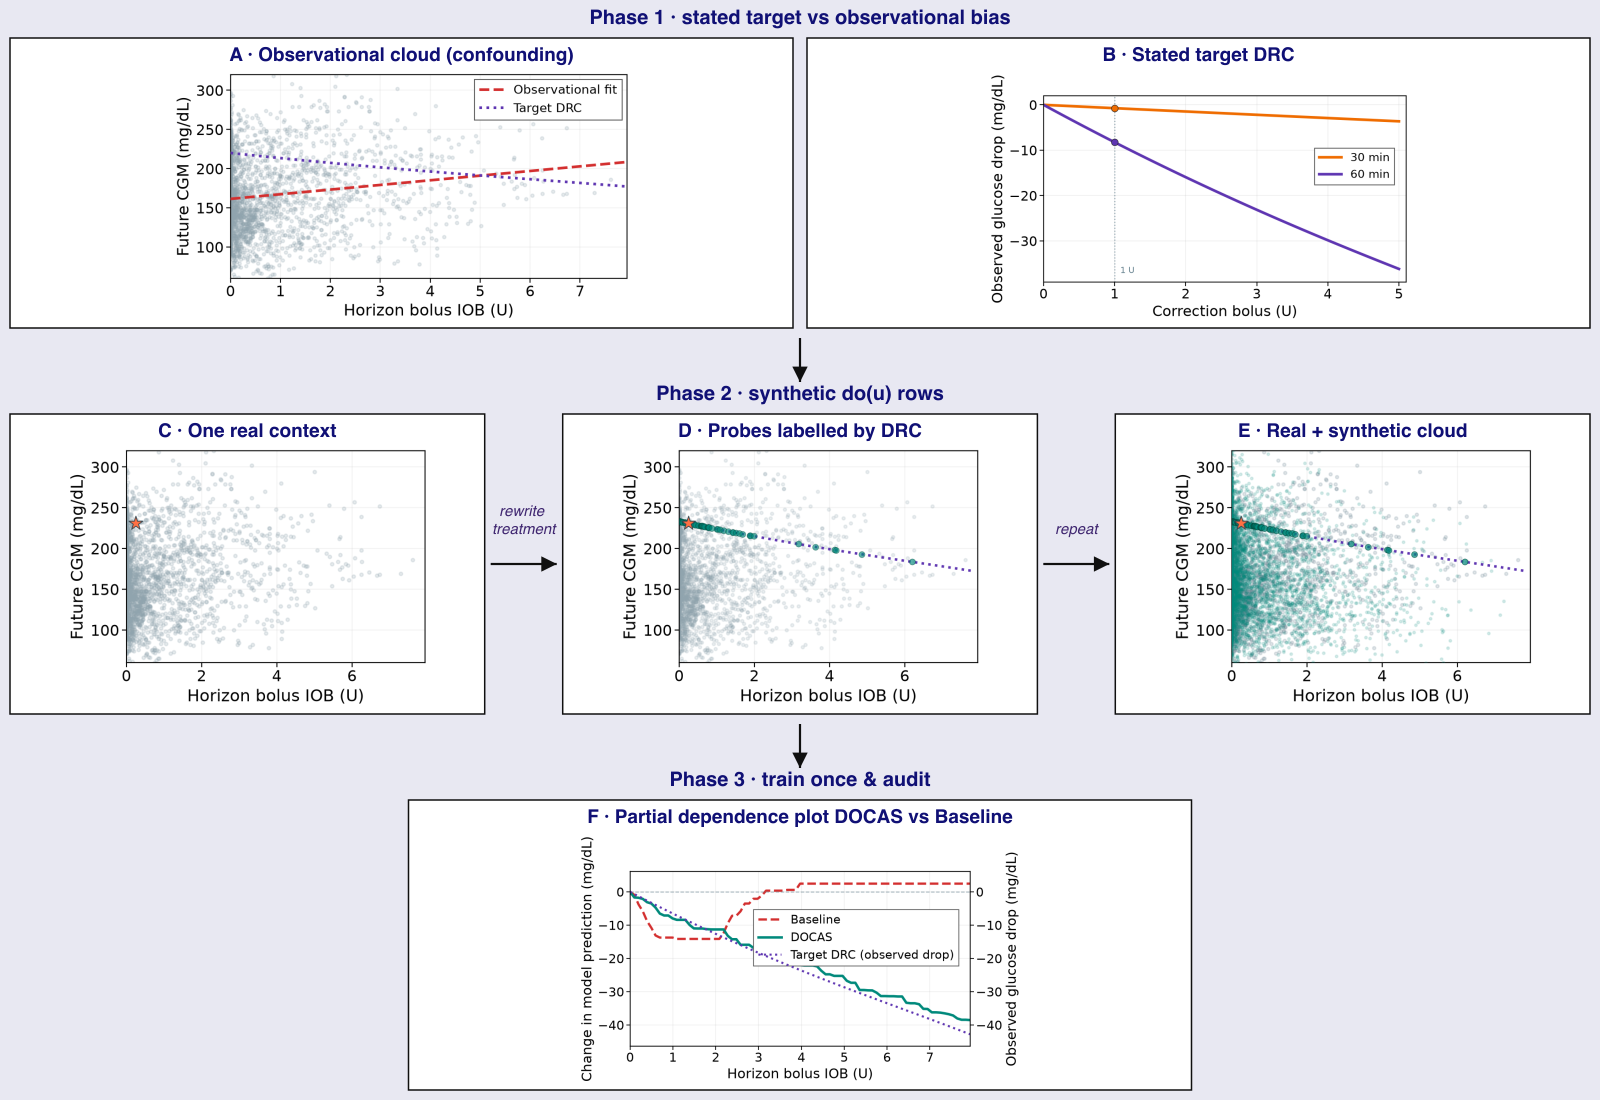
\includegraphics[width=\textwidth]{figures/docas_flowchart.png}
  \caption{Overview of the DOCAS alignment procedure across three phases
  (illustrated on OhioT1DM patient~588).
  \textbf{Phase~1.} \textbf{A:} observational training distribution exhibiting
  treatment-indication confounding, contrasted with the slope of the target
  DRC. \textbf{B:} stated target DRC at 30 and 60 minutes. Its vertical axis is
  the observed glucose drop when that dose is taken.
  \textbf{Phase~2.} \textbf{C--E:} counterfactual instance generation: copying
  observed contexts, sweeping the treatment feature across probe doses, and assigning
  labels via the factual outcome plus the incremental target DRC effect.
  \textbf{Phase~3.} \textbf{F:} partial dependence plot (mean ICE across test
  contexts) of DOCAS versus Baseline (original training records only). Its
  vertical axis is the change in the model's prediction. A second vertical axis
  shows the target DRC, the observed drop those predictions are compared with.}
  \label{fig:flowchart}
\end{figure*}

\subsection{Conceptual formulation}
\label{subsec:docas-concept}

A supervised model is trained on observational records, each of which pairs a
context---all input features other than the treatment---with the dose that was
actually given and a continuous outcome. Empirical risk minimization fits the
observational association between those inputs and the outcome. When higher
doses are reserved for more severe cases, that association can run opposite to
the drug's biological effect: more treatment then predicts a worse outcome.
Figure~\ref{fig:flowchart}A shows this for insulin: in the observed data, future glucose rises with
insulin on board (red dashed line), whereas the target DRC (dotted line) falls.

Decision support asks a different question: it requires the prediction that
would follow from setting the treatment while holding the context
fixed. Sweeping the treatment feature across a dose range,
with all other features of that record unchanged, yields an individual
conditional expectation (ICE): one curve per context, reported as the change in
prediction relative to the value at null
dose~\citep{goldstein2015}. Dose is normalised to the unit interval using a
domain-specific maximum. A partial dependence plot (PDP) averages these
curves over many contexts and can hide opposing slopes.

The \emph{target DRC} is the expected dose--response from
mechanistic principles or clinical consensus. It is a stated prior, not
patient-specific ground truth, because the true interventional response is not
observed in static logs. \emph{Alignment error} (AE) is the root-mean-square
gap between each of those ICEs and the target DRC, taken over all evaluation
contexts and a dense grid of doses:
\begin{equation}
  \mathrm{AE}
  \;=\;
  \sqrt{\mathrm{mean}\bigl[(\text{ICE}-\text{DRC})^{2}\bigr]}.
  \label{eq:alignment-error}
\end{equation}
AE uses the physical units of the outcome, while held-out RMSE measures factual
accuracy on observational test data.

\subsection{Generic DOCAS framework}
\label{subsec:docas-generic}

\paragraph{Phase 1: defining the target DRC and context.}
We define the target DRC as the expected change in outcome when treatment is
set to a given dose, holding the remaining inputs---the context---fixed.
Because observational datasets rarely cover wide dose sweeps
under uniform contexts, the target DRC supplies the missing interventional
supervision. Figure~\ref{fig:flowchart}B shows the target DRC used in this study, i.e.\ the
observed glucose drop 30 and 60 minutes after a correction bolus of a given size.

\paragraph{Phase 2: generating synthetic counterfactual instances.}
In Phase~2, DOCAS adds synthetic training rows that show the model how the
outcome changes when only the dose changes; the observed rows are kept as they
are. \hl{The number of synthetic rows is a multiple of the number of observed
training rows, which we call the synthetic budget.} In this study, a budget of 20, i.e.\ twenty synthetic rows per
observed row, was selected on validation data (Section~\ref{subsec:ablation}).
Each synthetic row is created as follows. First, a real training row is drawn
at random, with replacement, and copied (star in Figure~\ref{fig:flowchart}C). It provides a
realistic context, i.e.\ a combination of current glucose, recent carbohydrates,
and other inputs that actually occurred. Second, small Gaussian noise is added
to the continuous context features (standard deviation of 10 for glucose in
mg/dL and carbohydrates in g, with glucose kept above 40~mg/dL and carbohydrates
non-negative), so that the many copies of one row do not show the model the
same context over and over again. Third, the dose is replaced by a probe dose
(green points in Figure~\ref{fig:flowchart}D). Half of the probe doses are drawn from the doses
observed in training (density-based sampling), so that common doses such as
small correction boluses are well represented. The other half are drawn
uniformly between zero and the maximum dose (uniform sampling), so that large
doses, which are rare in the logs, are covered as well.

Finally, each synthetic row is labelled with the observed outcome of the copied
row plus the difference in the target DRC between the probe dose and the dose
that was actually given. For example, if the target DRC states that the probe
dose lowers glucose by 15~mg/dL more than the given dose, the label is the
observed glucose change minus 15~mg/dL. Everything apart from the dose that
influenced the observed outcome, e.g.\ a meal or sensor noise, thus remains in
the label, and the labelled probes lie on the target DRC through the copied
context (Figure~\ref{fig:flowchart}D). Repeating these steps for many contexts yields the
combined cloud of real and synthetic rows in Figure~\ref{fig:flowchart}E.

\paragraph{Phase 3: model training and evaluation.}
The synthetic rows are pooled with the observational data, and the same
supervised model is trained once on the combined set, using its native loss,
with no extra penalty terms and no change to the architecture. Performance is
evaluated on held-out test data via RMSE and via AE on the ICE of every test
context (Eq.~\ref{eq:alignment-error}). In Figure~\ref{fig:flowchart}F, the partial
dependence plot of the baseline, trained on the observed rows only, is flat or
rises at higher doses, whereas that of DOCAS follows the target DRC.

\subsection{Application to type~1 diabetes}\label{subsec:target}

We instantiate DOCAS for postprandial glucose forecasting on OhioT1DM
(open-loop pump therapy) and AZT1D (closed-loop automated insulin delivery;
cohort protocol in Section~\ref{subsec:ohio-protocol}), with bolus insulin on
board (IOB) as the treatment feature, basal insulin left unmanipulated, and the
30- or 60-minute change in continuous glucose monitor (CGM) readings as the
outcome.

The target DRC is the interstitial glucose drop of a rapid-acting correction
bolus, simulated in the UVa/Padova model as implemented in
ReplayBG~\citep{cappon2023,bergman1979} and scaled by the patient's current
glucose so that the same dose lowers glucose more when ambient glycaemia is
higher; both cohorts use this construction. Simulation settings, sensor
profiles, and the normalised dose axis are given in
Appendix~\ref{app:target-data}. Figure~\ref{fig:iob-pharmacology} shows the
simulated trajectory and the resulting target DRC.

\begin{figure*}[!htbp]
  \centering
  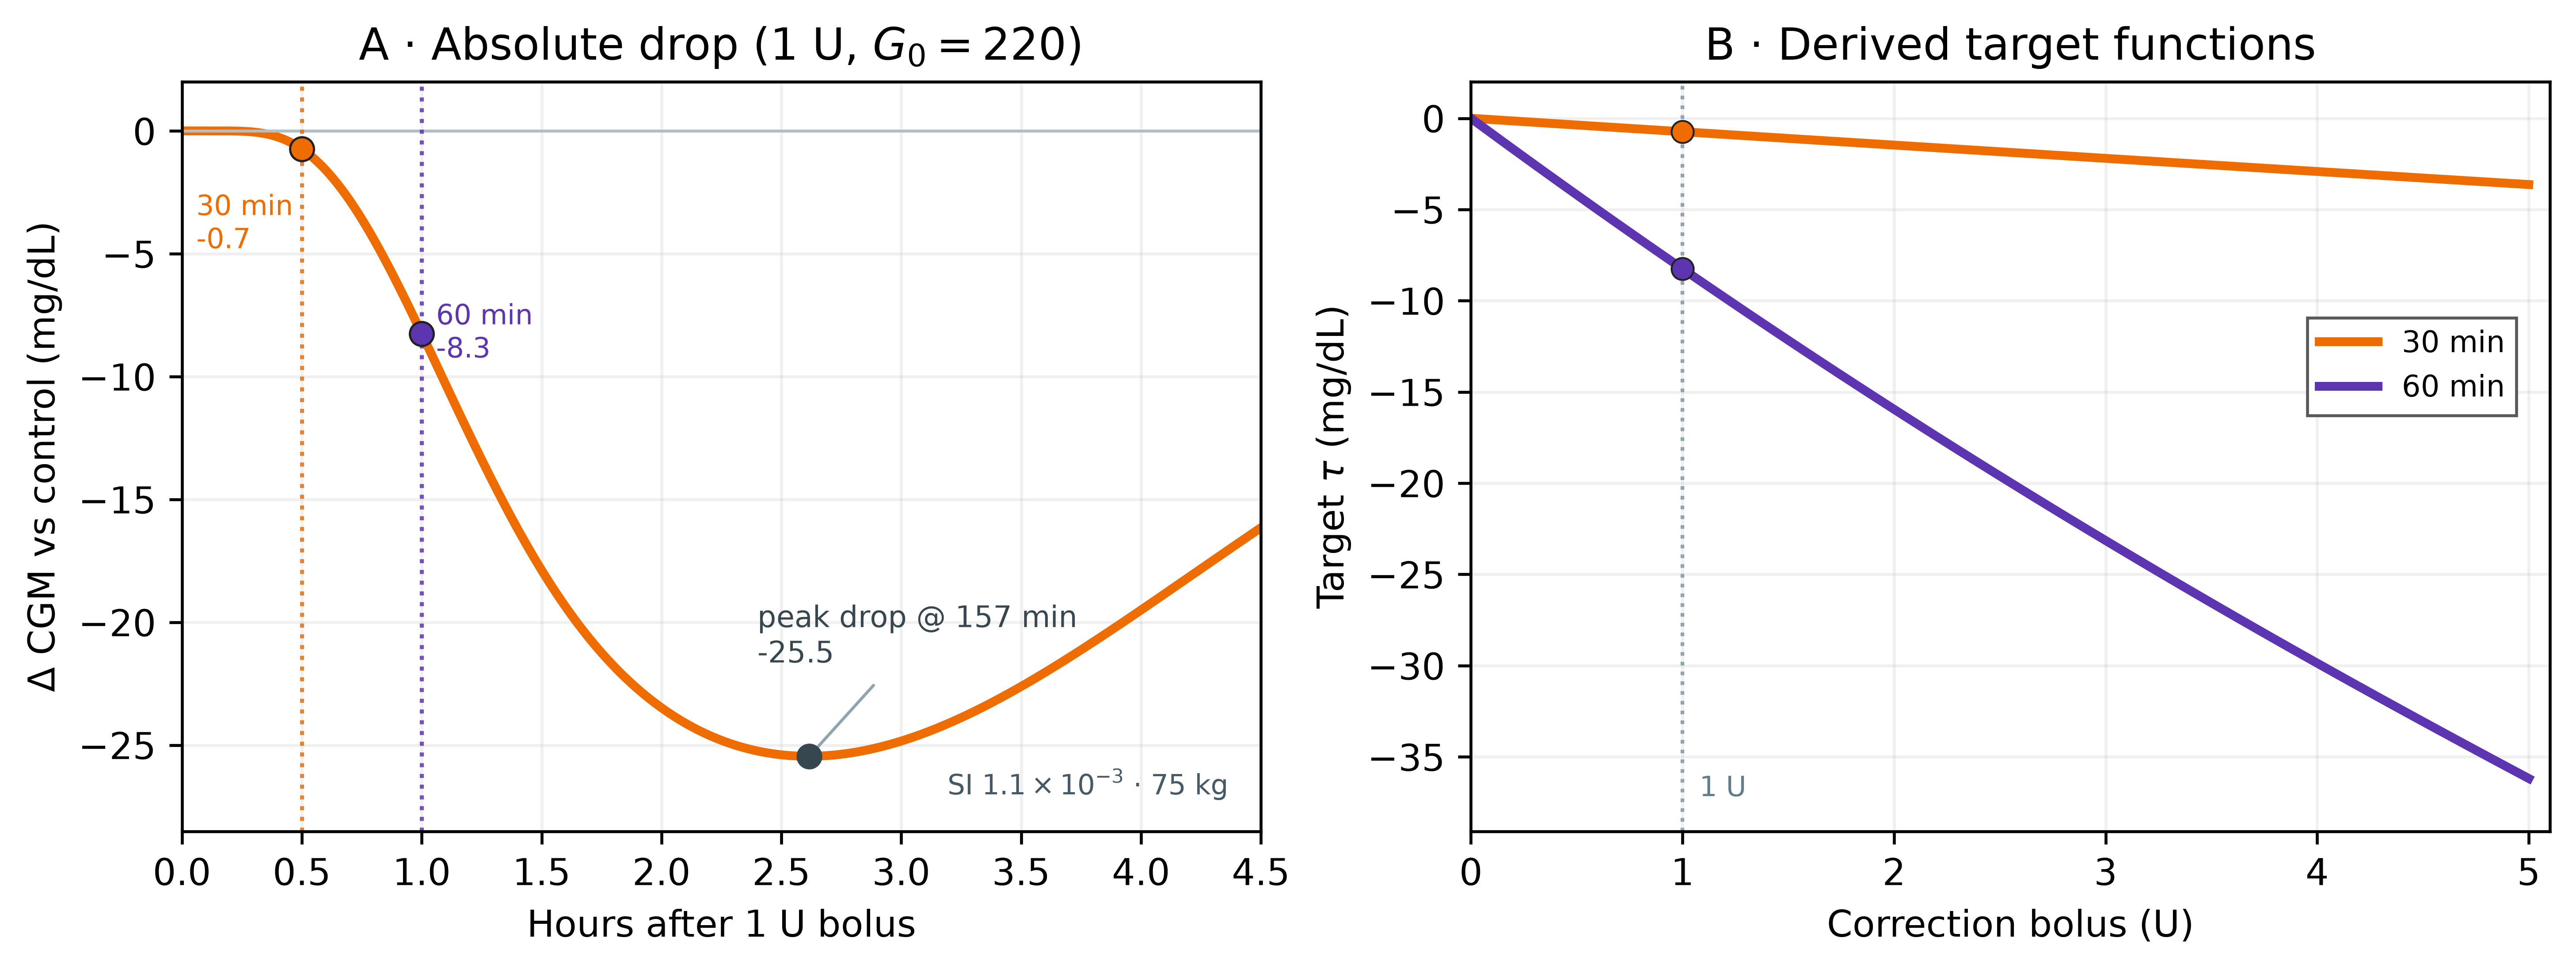
\includegraphics[width=0.92\textwidth]{figures/iob_pharmacology.png}
  \caption{Ambient-scaled target DRC derived from ReplayBG simulation.
  \textbf{A:} interstitial glucose reduction following a 1~U bolus versus no-bolus
  control at $G_0{=}220$~mg/dL, indicating the drop at 30- and 60-minute
  horizons.
  \textbf{B:} derived target functions versus correction bolus across prediction
  horizons (1~U reference marked at baseline ambient glycaemia).}
  \label{fig:iob-pharmacology}
\end{figure*}

\subsection{Experimental setup and evaluation protocol}\label{subsec:ohio-protocol}

Our evaluation adopts the protocol of Prendin et al.~\citep{prendin2023}: identical
OhioT1DM train/test splits, IOB and carbohydrate on board (COB)
features, and the ReplayBG in-silico decision-support benchmark. Models map current
CGM, bolus IOB, and COB to future CGM change over 30- or 60-minute horizons. For
OhioT1DM ($n{=}12$), the initial six monitoring weeks serve as training data and the
final ten days are held out for testing~\citep{marling2020,prendin2023}. On-board
features use causal event histories available at forecast time.

We evaluate performance across cohorts via mean~$\pm$~standard deviation of
held-out RMSE and alignment error (AE) across all test contexts and a dense
dose grid from none to the domain maximum (Eq.~\ref{eq:alignment-error}). The primary
model architecture is CatBoost~\citep{prokhorenkova2018}. Baseline is the same
learner trained only on the original training records; DOCAS is trained on those
records plus the synthetic rows of Phase~2 (Appendix~\ref{app:target-data},
$20\times$ budget, 50\%/50\% empirical/uniform mix). Appendix~\ref{app:mlp} repeats the comparison for a multilayer
perceptron (MLP) and for CatBoost with 12 five-minute lags per channel (36 inputs).

The AZT1D dataset~\citep{khamesian2025azt1d,khamesian2025azt1ddata} provides an
external validation cohort of 24 participants on automated insulin delivery (Tandem
t:slim~X2 Control-IQ with Dexcom~G6~Pro). Subject~14 is excluded due to lack of an
isolated CGM channel. We employ an 80/20 chronological
split per patient, matching feature definitions, the target DRC of
Appendix~\ref{app:target-data}, and evaluation metrics.

Statistical significance between baseline and DOCAS arms is evaluated using paired,
two-sided Wilcoxon signed-rank tests across patients with Holm--Bonferroni correction
($\alpha{=}0.05$). CatBoost employs untuned default parameters (depth~6, automatic
learning rate, 1000-iteration maximum) with early stopping (patience~50) evaluated
on a chronological 20\% validation split of each arm's training distribution. Primary
results in Table~\ref{tab:prediction} and the MLP rows of Appendix~\ref{app:mlp} report averages over
five random seeds ($42$--$46$); the lag-feature rows, ablations, and parameter sweeps use seed~$42$.

\section{Results}\label{sec:results}

\subsection{Held-out accuracy and alignment}\label{subsec:ohio-results}

Figure~\ref{fig:drc} shows the insulin PDP of each patient, i.e.\ the mean of
the ICE curves over the patient's test contexts. The baseline CatBoost, trained
only on the original records, produced curves that were flat or even increased
with insulin, which is the pattern expected from treatment-indication
confounding. With DOCAS, the curves decreased with insulin and followed the
stated DRC for both horizons. Table~\ref{tab:prediction} gives the cohort
averages over five seeds.

In both cohorts, DOCAS reduced the alignment error by $89$--$93\%$ compared
with the baseline, while the RMSE increased by only $2.7$--$4.4\%$. On
OhioT1DM, AE decreased from $12.70$~mg/dL (baseline) to $1.44$~mg/dL (DOCAS) at
30~minutes and from $38.13$ to $2.79$~mg/dL at 60~minutes, with an RMSE
increase of $3.2\%$ and $4.4\%$. For AZT1D, AE decreased from $19.62$ to
$1.70$~mg/dL and from $49.30$ to $4.13$~mg/dL, with an RMSE increase of $2.7\%$
and $3.0\%$. Alignment improved for every participant in both cohorts, and the
reductions were significant for all cohorts and horizons (paired Wilcoxon tests
with Holm--Bonferroni correction). The same was observed for an MLP, and adding
lag features reduced the DOCAS alignment error even further
(Appendix~\ref{app:mlp}).

\begin{figure*}[!htbp]
  \centering
  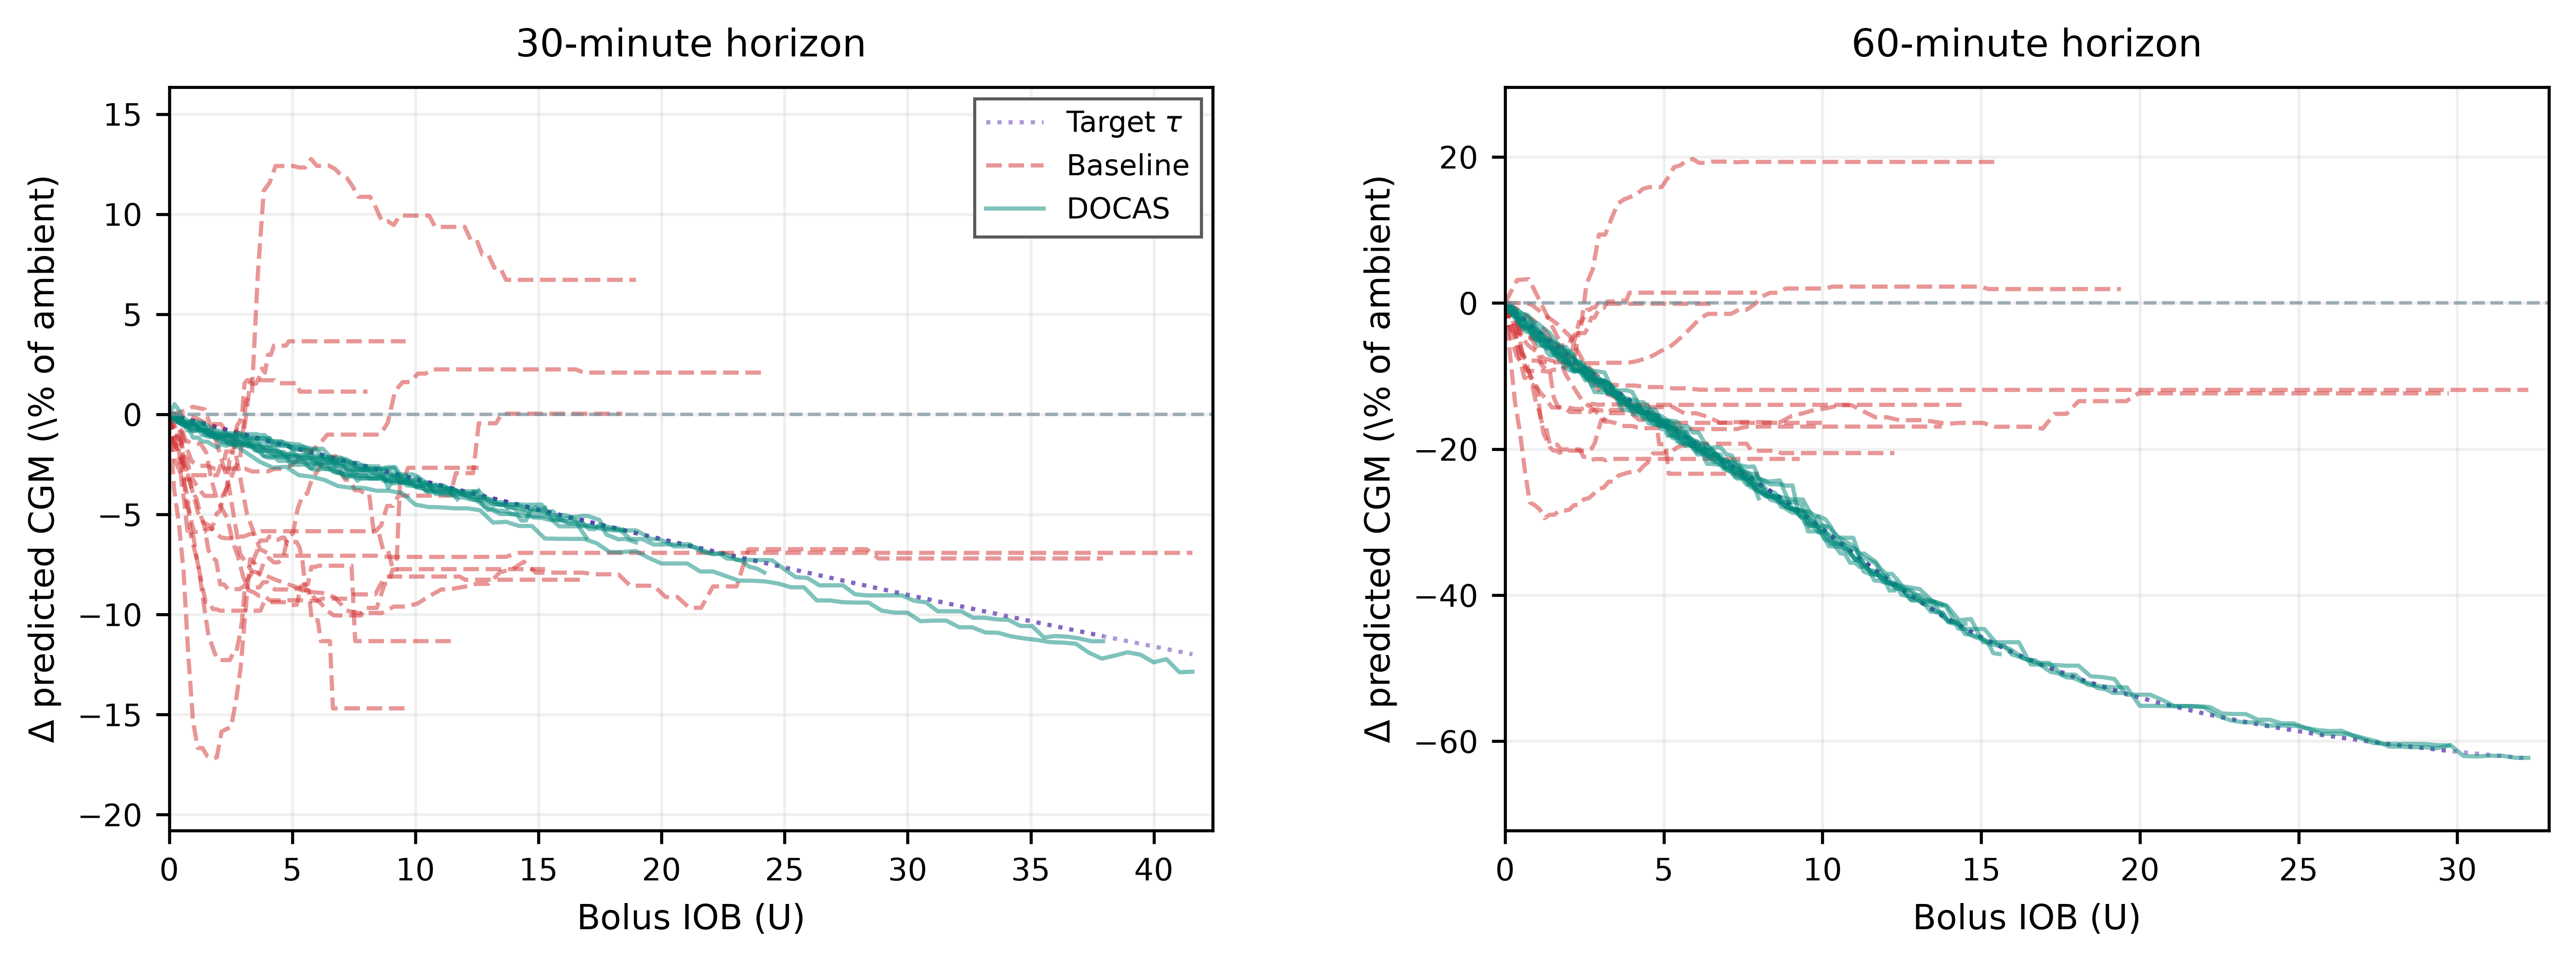
\includegraphics[width=\textwidth]{figures/dose_response_curves.png}
  \caption{Patient-level insulin PDP on OhioT1DM (mean ICE per patient).
  Alignment error in Table~\ref{tab:prediction} is evaluated on the per-context ICE
  versus the target DRC.
  $\Delta$ predicted CGM expressed as \% of mean test ambient CGM.
  \textbf{Left:} 30-minute horizon; \textbf{right:} 60-minute horizon. Curves extend
  to each patient's training-maximum IOB.}
  \label{fig:drc}
\end{figure*}

The results on participant level are consistent with these averages. On
OhioT1DM, even the participant with the smallest improvement reduced AE by more
than 4~mg/dL at 30~minutes and by almost 14~mg/dL at 60~minutes. Since the
synthetic rows are only used for training and AE is evaluated on held-out test
contexts, this shows that the learned insulin response generalizes to unseen
situations. For dosing, the 60-minute horizon is the more relevant one, since
after 30~minutes a bolus has lowered glucose only slightly, often by less than
the sensor noise.

The RMSE cost was small for all participants. DOCAS even lowered the RMSE for 2
of 12 OhioT1DM participants at 30~minutes and for 3 of 12 at 60~minutes, and for
every participant the increase in RMSE was less than a quarter of the AE
improvement. Note that the RMSE measures how well the forecaster predicts
glucose when nothing is changed, while the ICE determines which dose it
recommends.

\FloatBarrier
\begin{table}[pos=htbp,width=\linewidth]
\centering
\caption{Held-out CatBoost RMSE and alignment error on both cohorts.
 Baseline: original training records only. DOCAS: original records plus
 synthetic Phase~2 rows. Cohort mean~$\pm$~SD over 5 seeds. Bold$^*$:
 significantly better arm (Section~\ref{subsec:ohio-protocol}). MLP and lag features in
 Appendix~\ref{app:mlp}.
}
\label{tab:prediction}
\scriptsize
\begin{tabular}{lcccc}
\toprule
 & \multicolumn{2}{c}{30 min} & \multicolumn{2}{c}{60 min} \\
\cmidrule(lr){2-3}\cmidrule(lr){4-5}
Approach & RMSE & Align. & RMSE & Align. \\
\midrule
\multicolumn{5}{@{}l}{\textbf{OhioT1DM} ($n=12$)} \\
Baseline & \textbf{21.91 $\pm$ 3.04}$^*$ & 12.70 $\pm$ 5.14 & \textbf{34.32 $\pm$ 4.35}$^*$ & 38.13 $\pm$ 22.19 \\
DOCAS & 22.61 $\pm$ 2.62 & \textbf{1.44 $\pm$ 0.67}$^*$ & 35.83 $\pm$ 3.64 & \textbf{2.79 $\pm$ 0.56}$^*$ \\
\addlinespace
\multicolumn{5}{@{}l}{\textbf{AZT1D} ($n=24$)} \\
Baseline & \textbf{21.60 $\pm$ 3.44}$^*$ & 19.62 $\pm$ 16.11 & \textbf{31.82 $\pm$ 5.55}$^*$ & 49.30 $\pm$ 29.29 \\
DOCAS & 22.19 $\pm$ 3.32 & \textbf{1.70 $\pm$ 0.84}$^*$ & 32.78 $\pm$ 5.18 & \textbf{4.13 $\pm$ 2.44}$^*$ \\
\bottomrule
\end{tabular}
\end{table}


\subsection{Investigating the alignment and prediction performance trade-off}
\label{subsec:trade-off}

Figure~\ref{fig:align-individual} illustrates the trade-off between alignment and
prediction performance. Among test hours where
DOCAS reduced the 60-minute forecast ($r=-0.50$, $n{=}14{,}993$), alignment improved
accuracy during glucose drops (mean absolute error improvement $4.49$; 88\% of
instances) and degraded accuracy during postprandial rises ($-5.14$; DOCAS superior
in 15\%). Participant~544 represents an extreme post-meal state: glucose rises from
$148$ to $232$~mg/dL. The observational model predicts this rise ($\approx 213$),
whereas DOCAS predicts $\approx 158$ based on active IOB. Conversely,
participant~563 represents an isolated correction without active carbohydrate: glucose
falls from $278$ to $200$~mg/dL, and DOCAS ($\approx 207$) outperforms the
observational baseline ($\approx 251$).

\begin{figure*}[!htbp]
  \centering
  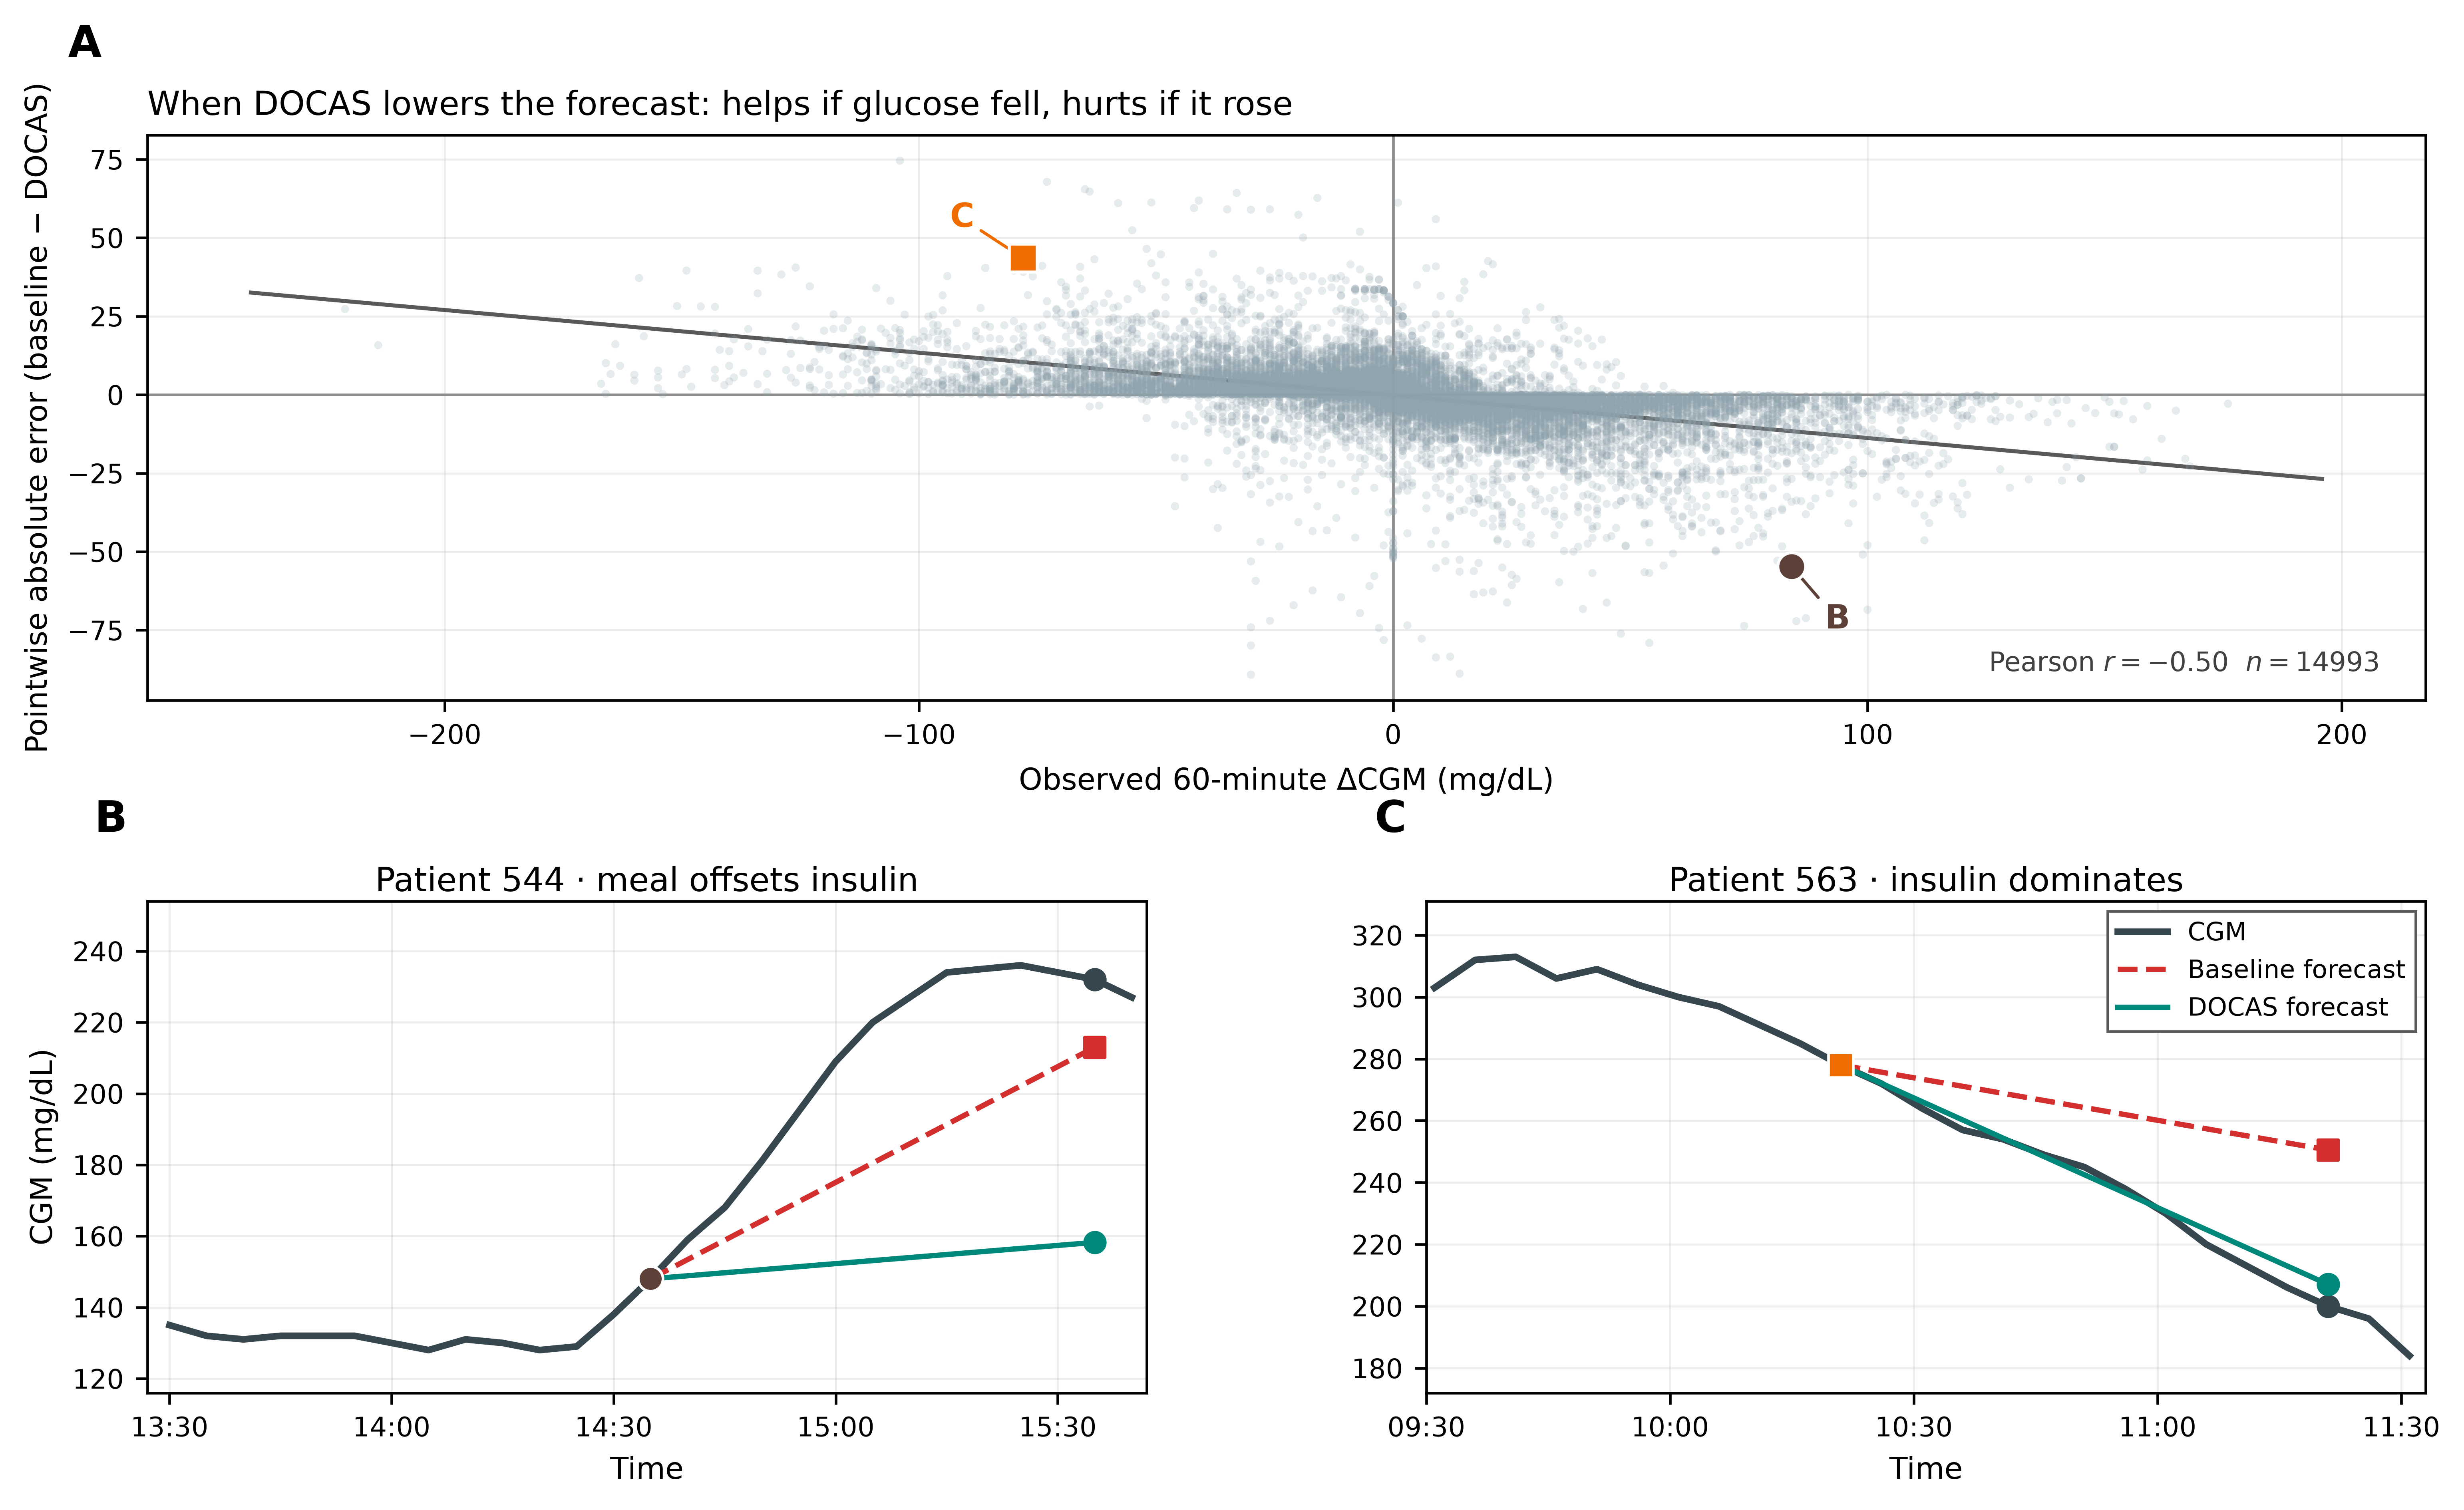
\includegraphics[width=\textwidth]{figures/alignment_individual.png}
  \caption{Evaluation of 60-minute predictions under aligned versus observational models.
  \textbf{A:} test hours where DOCAS lowered the prediction: observed $\Delta$CGM
  versus pointwise absolute-error improvement (baseline minus DOCAS; Pearson $r{=}-0.50$,
  $n{=}14{,}993$; markers B and C denote instances in panels B and C).
  \textbf{B:} participant~544 (meal absorption counteracting insulin action).
  \textbf{C:} participant~563 (insulin-dominated glucose decline).}
  \label{fig:align-individual}
\end{figure*}

\subsection{In-silico decision support}\label{subsec:replay-results}

We integrate each trained model into the corrective-bolus decision support system
(DSS) of Prendin et al.~\citep{prendin2023} and evaluate outcomes in silico using
ReplayBG~\citep{cappon2023}: a physiological simulator fitted to real glucose--insulin
trajectories, replaying identical episodes under alternative dosing policies. The
protocol evaluates all 12 OhioT1DM participants under matched conditions. AZT1D is
omitted from replay because its automated Control-IQ algorithm already issues
closed-loop corrections (median $35.6\%$ automatic boluses, $41.4\%$ automated basal
modulation), confounding independent DSS evaluation.

The benchmark isolates eight-hour postprandial windows without subsequent carbohydrate
or manual boluses. Two hours post-meal, if glucose exceeds $180$~mg/dL, the DSS
evaluates candidate boluses from $0$ to $5$~U in 0.5~U increments, minimizing the
squared deviation from a $120$~mg/dL target at 60~minutes with a quadratic dose
penalty~\citep{prendin2023}. If no dose improves on zero, no bolus is given; a
second trigger is permitted after 120~minutes. To address the fact that only $\approx 20\%$
of rapid-acting insulin acts within 60~minutes, we incorporate an explicit
hypoglycaemia safety guard (Appendix~\ref{app:unguarded}, Figure~\ref{fig:safety}):
candidates are admissible only if their projected 180-minute nadir remains above
$70$~mg/dL. Rejected candidates step down to the highest admissible lower dose.

Windows qualify if the twin fits recorded glucose (RMSE~$\le 25$~mg/dL), baseline
replay exhibits hyperglycaemia, and a 1~U probe bolus yields a clinically plausible
drop ($\le 100$~mg/dL, nadir $\ge 70$~mg/dL). Eleven eligible windows across four
participants met all criteria; nine triggered active dosing (Table~\ref{tab:replay}).

Post-decision time in range (TIR, $70$--$180$~mg/dL) is $61.49\%$ with no
decision support, $73.61\%$ under Baseline (mean dose $1.09$~U), and
$76.01\%$ under DOCAS (mean dose $2.23$~U), with zero time below range
(TBR, $<70$~mg/dL) across all arms under the safety guard. The paired TIR
improvement is $+2.40$~percentage points (pp) across windows
($p{=}0.062$, positive in all five windows where TIR differed).
Sweeping the dose penalty confirms
that DOCAS maintains higher TIR across operating points: the observational DSS plateaus
at $1.41$~U due to its upward-sloping ICE, whereas DOCAS scales from
$0.73$ to $2.32$~U. At matched dosing ($\sim 1.09$~U) the arms are
comparable, confirming that alignment enables safe, larger therapeutic
corrections.

Across the nine triggering decision points, the observational ICE deviates by a mean
of $17.27$~mg/dL from the target curve, whereas DOCAS deviates by $1.83$~mg/dL. At
a 5~U probe, the observational model predicts a $7.02$~mg/dL glucose \emph{increase},
whereas the target DRC specifies a $25.40$~mg/dL drop and DOCAS predicts a
$26.39$~mg/dL drop. The DOCAS ICE is strictly non-increasing across all nine
decisions, compared to once for the baseline.
Figure~\ref{fig:ohio-replay} shows one window for OhioT1DM patient~588: the
observational ICE turns upward beyond $2.5$~U and the DSS picks $0.5$~U,
whereas DOCAS follows the target DRC and picks $2.0$~U.

\FloatBarrier
\begin{table}[pos=htbp,width=0.72\linewidth]
\centering
\caption{Post-decision outcomes for no decision support and the two corrective-bolus policies on 11 OhioT1DM windows from 4 participants (mean~$\pm$~SD).}
\label{tab:replay}
\scriptsize
\begin{tabular}{lccc}
\toprule
Metric & No DSS & Baseline & DOCAS \\
\midrule
TBR (\%) & 0.00 $\pm$ 0.00 & 0.00 $\pm$ 0.00 & 0.00 $\pm$ 0.00 \\
TIR (\%) & 61.49 $\pm$ 34.22 & 73.61 $\pm$ 23.83 & 76.01 $\pm$ 21.95 \\
TAR (\%) & 38.51 $\pm$ 34.22 & 26.39 $\pm$ 23.83 & 23.99 $\pm$ 21.95 \\
Insulin (U) & 0.00 $\pm$ 0.00 & 1.09 $\pm$ 1.41 & 2.23 $\pm$ 2.04 \\
\bottomrule
\end{tabular}
\end{table}


\begin{figure*}[!htbp]
  \centering
  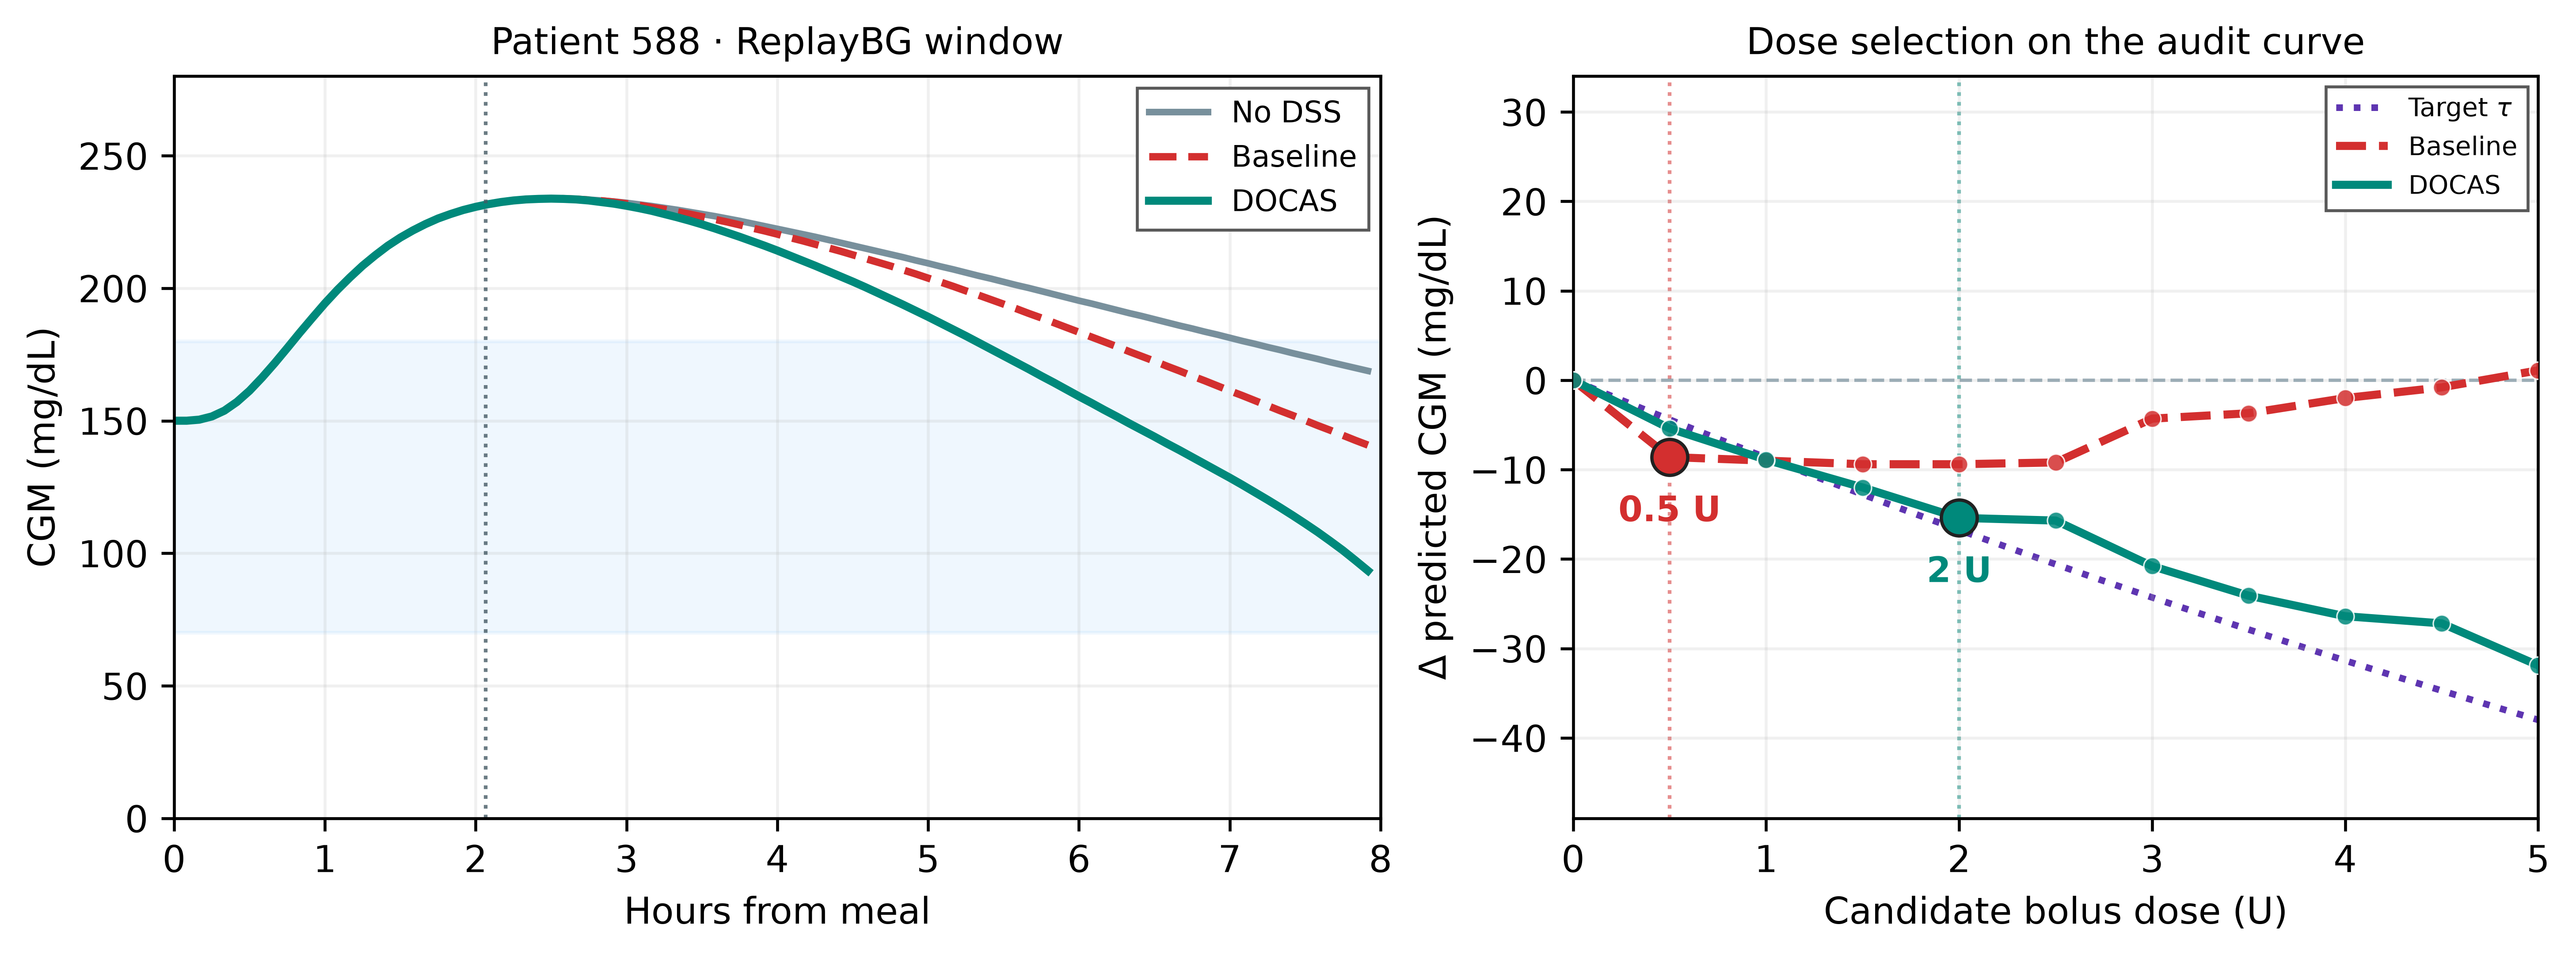
\includegraphics[width=0.92\textwidth]{figures/patient588_replay_window.png}
  \caption{In-silico postprandial replay for OhioT1DM patient~588 (CatBoost,
  60-minute horizon).
  \textbf{Left:} simulated glucose trajectories without DSS and under observational
  versus DOCAS-guided dosing.
  \textbf{Right:} decision-context ICE (marker denotes selected dose).
  The observational ICE turns upward beyond $2.5$~U ($0.5$~U chosen); DOCAS conforms
  to the target DRC ($2.0$~U chosen). Post-decision time in range increases from
  $13.89\%$ (No DSS) and $30.56\%$ (Baseline) to $44.44\%$ (DOCAS), with zero
  time below range.}
  \label{fig:ohio-replay}
\end{figure*}

\subsection{Ablation studies}\label{subsec:ablation}

We ablate four parts of the method on both cohorts (CatBoost, seed~$42$;
Table~\ref{tab:ablation}): how many synthetic rows are added, how probe doses
are drawn, whether the target DRC can be added after training instead of
during it, and whether the stated curve itself can be changed.

The study preset uses twenty synthetic rows per observed training row
($20\times$). A $0.1\times$ budget already cuts 30-minute AE ($9.23$ vs.\
$12.70$~mg/dL on OhioT1DM; $8.21$ vs.\ $19.62$~mg/dL on AZT1D) at essentially
no RMSE cost. At $1\times$, AE is $4.62$/$9.50$ and $4.48$/$8.12$~mg/dL. The
$20\times$ preset reaches $1.51$/$2.75$ and $1.64$/$3.64$~mg/dL; $100\times$
tightens AE further ($0.82$/$2.13$ and $0.84$/$2.32$~mg/dL) with only a small
extra RMSE rise. More synthetic rows therefore pull the per-context ICEs closer to the
target, at a small factual cost.

Probe doses in the study mix are half from the training dose density and half
uniform on $[0,1]$. Drawing every synthetic IOB uniformly instead leaves AE
much higher ($7.37$/$11.13$~mg/dL on OhioT1DM; $3.31$/$7.27$~mg/dL on AZT1D)
at almost the same RMSE, so coverage of common clinical doses matters.

Adding the target DRC after a no-insulin fit, rather than training on synthetic
rows, forces $\mathrm{AE}{=}0$ but raises 60-minute RMSE ($39.03$ vs.\ $35.80$
on OhioT1DM; $36.81$ vs.\ $32.82$ on AZT1D) and cannot change the recommended
dose with context, so alignment has to enter during training.

Scaling the prior insulin
sensitivity $S_I$ by $0.5\times$ or $2\times$ keeps AE in the same few mg/dL,
so the method follows the stated curve rather than a fixed amplitude. Replacing
UVa/Padova DRC with a pump-settings curve
(Eq.~\ref{eq:pump-tau}, Appendix~\ref{app:clinical-tau}) still aligns, with RMSE
$0.31$ (OhioT1DM, 30~min) and $0.72$ (AZT1D, 60~min) above the $20\times$
UVa/Padova run.

\begin{table}[pos=htbp,width=\linewidth]
\centering
\caption{Ablations on both cohorts (mean~$\pm$~SD, seed~$42$). Synthetic budgets $0.1\times$, $1\times$, and $100\times$ versus the study preset $20\times$. Uniform IOB only draws every probe from $\mathrm{Uniform}[0,1]$ (no training-density mix). The last row uses a pump-settings DRC (Section~\ref{subsec:ablation}).}
\label{tab:ablation}
\scriptsize
\resizebox{\linewidth}{!}{%
\begin{tabular}{lcccccccc}
\toprule
 & \multicolumn{4}{c}{OhioT1DM ($n=12$)} & \multicolumn{4}{c}{AZT1D ($n=24$)} \\
\cmidrule(lr){2-5}\cmidrule(lr){6-9}
 & \multicolumn{2}{c}{30 min} & \multicolumn{2}{c}{60 min} & \multicolumn{2}{c}{30 min} & \multicolumn{2}{c}{60 min} \\
\cmidrule(lr){2-3}\cmidrule(lr){4-5}\cmidrule(lr){6-7}\cmidrule(lr){8-9}
Ablation & Align. & RMSE & Align. & RMSE & Align. & RMSE & Align. & RMSE \\
\midrule
DOCAS ($20\times$ budget) & 1.51 $\pm$ 0.82 & 22.59 $\pm$ 2.62 & 2.75 $\pm$ 0.77 & 35.80 $\pm$ 3.64 & 1.64 $\pm$ 0.84 & 22.20 $\pm$ 3.33 & 3.64 $\pm$ 2.22 & 32.82 $\pm$ 5.21 \\
Budget $0.1\times$ & 9.23 $\pm$ 3.21 & 21.87 $\pm$ 3.00 & 20.41 $\pm$ 8.08 & 34.47 $\pm$ 4.15 & 8.21 $\pm$ 3.28 & 21.64 $\pm$ 3.44 & 16.29 $\pm$ 6.88 & 31.78 $\pm$ 5.47 \\
Budget $1\times$ & 4.62 $\pm$ 1.13 & 22.08 $\pm$ 2.87 & 9.50 $\pm$ 2.54 & 34.99 $\pm$ 3.86 & 4.48 $\pm$ 1.70 & 21.78 $\pm$ 3.38 & 8.12 $\pm$ 3.10 & 32.20 $\pm$ 5.44 \\
Budget $100\times$ & 0.82 $\pm$ 0.42 & 22.69 $\pm$ 2.59 & 2.13 $\pm$ 0.96 & 35.96 $\pm$ 3.57 & 0.84 $\pm$ 0.58 & 22.32 $\pm$ 3.28 & 2.32 $\pm$ 1.85 & 33.11 $\pm$ 5.06 \\
Uniform IOB only & 7.37 $\pm$ 4.26 & 22.48 $\pm$ 2.65 & 11.13 $\pm$ 6.74 & 35.73 $\pm$ 3.62 & 3.31 $\pm$ 1.23 & 22.12 $\pm$ 3.35 & 7.27 $\pm$ 3.56 & 32.61 $\pm$ 5.30 \\
DRC applied after prediction & 0.00 $\pm$ 0.00 & 22.79 $\pm$ 2.59 & 0.00 $\pm$ 0.00 & 39.03 $\pm$ 5.36 & 0.00 $\pm$ 0.00 & 22.45 $\pm$ 3.21 & 0.00 $\pm$ 0.00 & 36.81 $\pm$ 8.38 \\
DRC at $0.5\times S_I$ & 1.57 $\pm$ 0.91 & 22.58 $\pm$ 2.72 & 2.68 $\pm$ 0.79 & 35.23 $\pm$ 3.85 & 1.66 $\pm$ 0.94 & 22.17 $\pm$ 3.35 & 3.35 $\pm$ 2.35 & 32.56 $\pm$ 5.30 \\
DRC at $2\times S_I$ & 1.48 $\pm$ 0.67 & 22.67 $\pm$ 2.44 & 4.48 $\pm$ 2.85 & 36.88 $\pm$ 3.83 & 1.61 $\pm$ 0.73 & 22.31 $\pm$ 3.29 & 4.57 $\pm$ 2.77 & 33.30 $\pm$ 5.26 \\
Clinical DRC (pump settings) & 1.58 $\pm$ 0.83 & 22.90 $\pm$ 2.26 & 2.70 $\pm$ 0.75 & 35.72 $\pm$ 3.44 & 1.99 $\pm$ 1.03 & 22.60 $\pm$ 3.21 & 4.56 $\pm$ 3.54 & 33.54 $\pm$ 5.60 \\
\bottomrule
\end{tabular}}
\end{table}


\section{Discussion}\label{sec:discussion}
\textit{Summary of results.}
This study aimed to evaluate and correct the insulin response of glucose forecasters trained on observational type~1 diabetes data. On OhioT1DM and AZT1D, DOCAS brought the insulin ceteris paribus plots close to the target DRC at a small RMSE cost, for every participant and for both CatBoost and an MLP (Table~\ref{tab:prediction}, Appendix~\ref{app:mlp}). Compared with the baseline, DOCAS reduced AE on OhioT1DM from $12.70$ to $1.44$~mg/dL at 30~minutes and from $38.13$ to $2.79$~mg/dL at 60~minutes (RMSE $+3.2\%$ and $+4.4\%$), and on AZT1D from $19.62$ to $1.70$~mg/dL and from $49.30$ to $4.13$~mg/dL (RMSE $+2.7\%$ and $+3.0\%$). In the ReplayBG evaluation, the ceteris paribus plot of the baseline turned upward beyond $2.5$~U and the corresponding DSS underdosed. The aligned forecaster, in contrast, stayed within $1.83$~mg/dL of the target curve, recommended $2.23$ instead of $1.09$~U on average, and increased the post-decision time in range from $73.61\%$ to $76.01\%$ with no time below range under the safety guard (Table~\ref{tab:replay}, Figure~\ref{fig:ohio-replay}).

\textit{Alignment error and synthetic data.}
A forecaster used for dosing has to answer how glucose changes if the dose changes and nothing else does, and the RMSE does not test this. In this study, every unaligned model responded to insulin with a flat or wrong-signed curve, including models with competitive RMSE. \hl{This can already be seen in the ceteris paribus plots. The AE, however, quantifies it, so that the insulin response can be reported next to the RMSE, compared across models and cohorts, and tracked when the synthetic budget changes} (Tables~\ref{tab:prediction} and~\ref{tab:replay}). Since DOCAS adds the target curve to the training data and not to the model, the same procedure could be used for CatBoost and an MLP without a custom loss, layer, or mechanistic component. A monotonic constraint would only have fixed the sign, and a monotone ceteris paribus plot that is too flat or too steep still leads to under- or overdosing~\citep{wolber2025,kushner2020,runje2023}. \hl{It is important to note that the target DRC and the associated AE by no means measure a deviation from an absolute ground truth.} The ceteris paribus plots of the patient's forecaster are compared with the same UVa/Padova curve, which describes the expected insulin action in a population and not in the individual patient~\citep{dallaman2007,cobelli2009}. We chose a population curve because an individual dose--response curve is hard to obtain. Insulin sensitivity varies between people and, within a person, with time of day and physical activity~\citep{hinshaw2013,visentin2015,riddell2017}. The observational logs cannot provide such a curve, since they are confounded in the way described above, and estimating it directly would require controlled dosing experiments that are rarely feasible in routine care. \hl{The population curve is therefore a distant, pharmacology-based reference, but aligning a forecaster to it may still be better than no alignment at all, since an unaligned forecaster can respond to insulin with the wrong sign.} Accordingly, a low AE shows that the forecaster responds to insulin as described by the population curve, but not that the pharmacology of the individual patient has been recovered.

\textit{Relation to mechanistic, hybrid, and mixed-effects models.}
\hl{Using a population mechanistic model as physiological basis for a data-driven model is an established strategy}~\citep{froehlich2018}, and DOCAS follows this strategy: the biology comes from UVa/Padova and is not learned from the logs. Synthetic labels, explicit integration, and a physics-informed loss can all encode this prior knowledge, but only explicit integration keeps the equations in the model and thereby the ability to extrapolate~\citep{fiedler2008,samadi2022,vonstosch2014}. DOCAS, in contrast, extrapolates only as far as the distribution of the synthetic data reaches. The forecaster learns the insulin response for dosing scenarios that are missing from the logs, but only within the range covered by the synthetic rows, i.e.\ doses between zero and the domain maximum in contexts close to the observed ones. \hl{Mechanistic, hybrid, and NONMEM-type mixed-effects models answer ceteris paribus dose questions within their structure and quantify the variability between subjects}~\citep{sheiner1980,mould2012,jones2013}. They are the better choice when the equations must hold exactly and have to extrapolate. DOCAS addresses a different setting, in which a data-driven forecaster trained on the patient's logs is used by a decision support system and its insulin response has to be checked and corrected. \hl{The DRC describes the population, whereas the observations are the patient's own glucose, meal, and insulin records. DOCAS combines both by training one model on the union of observed and synthetic rows. In this way, the population curve determines the insulin response, while the observations shape everything else the forecaster learns about the patient.} Since the prior knowledge enters only through training rows that compete with the observed data, the ceteris paribus plots of DOCAS do not match the target DRC exactly. In contrast, a wrapper that adds the DRC after prediction to a forecaster trained without insulin matches the target DRC exactly by construction (AE${}=0$). However, this wrapper predicts glucose worse than DOCAS, with a 60-minute RMSE of $39.03$ instead of $35.80$~mg/dL on OhioT1DM and $36.81$ instead of $32.82$~mg/dL on AZT1D (Table~\ref{tab:ablation}). DOCAS therefore accepts a small AE in exchange for a better fit. \hl{Learning from the observations and the population curve together therefore results in a better fit of the patient's glucose than adding the curve afterwards.}

\textit{Limitations.}
In the main study, only one target was used, the UVa/Padova DRC derived from ReplayBG. The same curve was used to label the synthetic rows and to compute the AE, and the in-silico decision support evaluation was run in ReplayBG, whose simulated patients follow the same model. The evaluation is therefore not independent of the target: a forecaster aligned to this curve is scored against the curve it was trained on and tested in a simulator built on the same pharmacology. We addressed this limitation directly with a second, realistic target DRC based on each participant's pump settings, i.e.\ the correction factor and the insulin action curve~\citep{walsh2011}. DOCAS trained on this pump-settings target still aligned and still improved decision support (Section~\ref{subsec:ablation}, Appendix~\ref{app:clinical-tau}), so the benefits are not tied to the UVa/Padova DRC. In-silico dosing was only evaluated on open-loop OhioT1DM records, since closed-loop automated insulin delivery in AZT1D continuously adjusts basal rates and delivers automated boluses, which confounds an external DSS evaluation. Furthermore, the absence of time below range depends on the explicit hypoglycaemia safety guard (Appendix~\ref{app:unguarded}). Since single-horizon forecasters capture only $\approx 20\%$ of rapid-acting insulin action at 60~minutes, an external constraint against late nadirs is necessary. Finally, the in-silico replay covered 11 postprandial windows across four eligible participants and therefore provides proof-of-concept evidence rather than the evidence of a clinical trial.

\textit{Future directions.}
Our first aim is a better trade-off between alignment and accuracy (Section~\ref{subsec:trade-off}). Better sampling of the synthetic rows could bring the ceteris paribus plots closer to the target without any cost in RMSE, or even with an improvement. \hl{Compared with the UVa/Padova simulator itself, the aligned forecaster predicts the next hour of glucose from the patient's own logs while responding to insulin as described by the population curve.} A next step would be to replace the population curve with the dose--response of each individual patient, estimated from the logs after adjusting for meals, time of day, and activity~\citep{hinshaw2013,riddell2017,cappon2023,prendin2025dt}. Type~1 diabetes was a suitable first application, since insulin pharmacodynamics are well characterized and public datasets with glucose, meal, and insulin logs are available. Beyond insulin, the approach can be applied to other treatments whenever a population dose--response for that input can be stated. An open-source implementation is available at \url{https://github.com/Prgrmmrjns/docas}.

\section{Conclusion}\label{sec:conclusion}

A glucose forecaster that is used to choose insulin doses should not only
predict glucose accurately but also respond correctly when the dose changes.
The held-out error only evaluates the former. In this study, we used the
alignment error to evaluate the latter by comparing the insulin response of the
forecaster with a population dose--response curve, and we introduced DOCAS,
which corrects this response by adding synthetic training rows without
changing the forecaster or replacing it with a mechanistic model. On two
type~1 diabetes cohorts, the aligned forecasters followed the target curve at a
small cost in accuracy. In silico, they recommended larger and more effective
correction boluses that increased the time in range without hypoglycaemia under
a safety guard.

\section*{Data availability}
OhioT1DM is distributed by the Ohio University College of Engineering under a
data-use agreement~\citep{marling2020}. AZT1D is publicly available as described by
Khamesian et al.~\citep{khamesian2025azt1d,khamesian2025azt1ddata}.
Processed features and result JSONs are reproduced from the accompanying code.

\section*{Code availability}
Source code to reproduce all tables and figures is available at
\url{https://github.com/Prgrmmrjns/DOCAS-manuscript}.
An implementation of the alignment procedure is available at
\url{https://github.com/Prgrmmrjns/docas}.

% Supplementary: MLP, lag features, unguarded CIB, clinical τ + ReplayBG.
\appendix

\section{Supplementary: target DRC and study data}\label{app:target-data}

OhioT1DM and AZT1D share one target DRC, obtained by simulating a rapid-acting
correction bolus against a matched no-bolus control from basal steady state in
ReplayBG~\citep{cappon2023} and recording the endpoint interstitial lowering at
horizon~$H$. Let $IG^{u}(H)$ and $IG^{\mathrm{ctl}}(H)$ denote interstitial
glucose under dose~$u$ and under the control. The fractional lowering and
ambient-scaled target DRC are
\begin{equation}
  \begin{aligned}
    R_H(u)
    &=
    \frac{1}{G_0}
    \bigl(IG^{\mathrm{ctl}}(H)-IG^{u}(H)\bigr),
    \\[0.35em]
    \tau_H(u;\,g)
    &=
    -g\,R_H(u).
  \end{aligned}
  \label{eq:target}
\end{equation}
Reference glucose is $G_0{=}220$~mg/dL. Body weight is $75$~kg. Insulin
sensitivity is the mode of ReplayBG's prior,
$S_I{=}1.15{\times}10^{-3}$~mL/($\mu$U$\cdot$min) (Gamma shape $\alpha{=}3.3$,
scale $5{\times}10^{-4}$). The remaining simulator values are the published
prior modes: glucose effectiveness $S_G{=}0.017$, insulin-action coupling
$p_2{=}0.11$, subcutaneous rates $k_d{=}0.021$~min$^{-1}$ and
$k_{a2}{=}0.011$~min$^{-1}$, elimination $k_e{=}0.127$~min$^{-1}$, volumes
$V_I{=}0.135$~dL/kg and $V_G{=}1.45$~dL/kg, and basal setpoint
$G_b{=}119$~mg/dL. Bolus lag is $8$~min on both cohorts. Sensor smoothing
follows the device: Enlite on OhioT1DM ($\alpha{=}10$) and Dexcom~G6 on AZT1D
($\alpha{=}5$). Figure~\ref{fig:iob-pharmacology} plots the simulated drop and
the resulting target DRC.

For forecasting, $u{=}1$ is each patient's training-maximum bolus insulin on
board. That span is often longer on AZT1D (closed-loop automated delivery) than
on OhioT1DM (open-loop pump therapy). The ReplayBG decision-support search
evaluates $0$--$5$~U. Cohort splits and features are in
Section~\ref{subsec:ohio-protocol}.

\section{Supplementary: MLP and lag features}\label{app:mlp}\label{app:lags}

Table~\ref{tab:prediction-mlp} repeats Table~\ref{tab:prediction} for a one-hidden-layer MLP (256 ReLU units, Adam, 100~epochs, learning rate $0.03$, batch size~512; five seeds) and for CatBoost with twelve five-minute lags per channel (36 inputs; 60~min history; one seed). The MLP insulin ICEs track the stated DRC at a small RMSE cost on both cohorts. The observational MLP starts further from the target than CatBoost, especially on AZT1D at 60~min, where long insulin-on-board spans stretch the normalised probe axis, and DOCAS closes that gap to the same few mg/dL. With the lags, RMSE falls for both arms, the baseline stays far from the stated DRC, and DOCAS alignment error is smaller than with instantaneous inputs.

\FloatBarrier
\begin{table}[pos=htbp,width=\linewidth]
\centering
\caption{MLP (five seeds) and CatBoost with twelve five-minute lags (one seed).
 Same protocol as Table~\ref{tab:prediction}. Cohort mean~$\pm$~SD.
 Bold$^*$: significantly better arm (Section~\ref{subsec:ohio-protocol}).}
\label{tab:prediction-mlp}
\label{tab:lags}
\scriptsize
\begin{tabular}{lcccc}
\toprule
 & \multicolumn{2}{c}{30 min} & \multicolumn{2}{c}{60 min} \\
\cmidrule(lr){2-3}\cmidrule(lr){4-5}
Approach & RMSE & Align. & RMSE & Align. \\
\midrule
\multicolumn{5}{@{}l}{\textbf{OhioT1DM} ($n=12$)} \\
MLP baseline & 22.23 $\pm$ 3.07 & 20.93 $\pm$ 8.48 & 35.41 $\pm$ 4.54 & 49.29 $\pm$ 25.25 \\
MLP DOCAS & 22.74 $\pm$ 2.62 & \textbf{1.89 $\pm$ 0.56}$^*$ & 36.33 $\pm$ 3.32 & \textbf{4.91 $\pm$ 0.75}$^*$ \\
\addlinespace
Lags baseline & \textbf{20.15 $\pm$ 2.36}$^*$ & 10.33 $\pm$ 6.83 & \textbf{32.88 $\pm$ 4.34}$^*$ & 42.97 $\pm$ 21.29 \\
Lags DOCAS & 21.82 $\pm$ 2.22 & \textbf{0.58 $\pm$ 0.17}$^*$ & 36.03 $\pm$ 3.88 & \textbf{2.36 $\pm$ 0.72}$^*$ \\
\addlinespace
\multicolumn{5}{@{}l}{\textbf{AZT1D} ($n=24$)} \\
MLP baseline & \textbf{21.96 $\pm$ 3.60}$^*$ & 39.74 $\pm$ 33.91 & \textbf{32.51 $\pm$ 5.66}$^*$ & 92.38 $\pm$ 69.86 \\
MLP DOCAS & 22.41 $\pm$ 3.24 & \textbf{2.14 $\pm$ 0.69}$^*$ & 33.42 $\pm$ 4.86 & \textbf{4.70 $\pm$ 1.17}$^*$ \\
\addlinespace
Lags baseline & \textbf{20.12 $\pm$ 3.50}$^*$ & 15.89 $\pm$ 15.65 & \textbf{30.44 $\pm$ 5.27}$^*$ & 46.42 $\pm$ 26.32 \\
Lags DOCAS & 21.89 $\pm$ 3.83 & \textbf{0.74 $\pm$ 0.40}$^*$ & 33.34 $\pm$ 6.19 & \textbf{2.03 $\pm$ 0.72}$^*$ \\
\bottomrule
\end{tabular}
\end{table}

\FloatBarrier

\section{Supplementary: hypoglycaemia guard}\label{app:unguarded}

As in Section~\ref{subsec:replay-results}, each candidate bolus on
$0$--$5$~U is scored on the ICE. Before a dose is suggested, the
60-minute predicted fall is scaled by the insulin still to act by 180~minutes
(about fourfold on the same insulin-action curve) and doubled, and the implied
nadir must stay above $70$~mg/dL; the doubling is a forecast-optimism margin. A
rejected candidate falls back to the next smaller admissible dose; both DSS
arms are checked identically. Figure~\ref{fig:safety} shows the loop on
patient~588.

\begin{figure*}[!htbp]
  \centering
  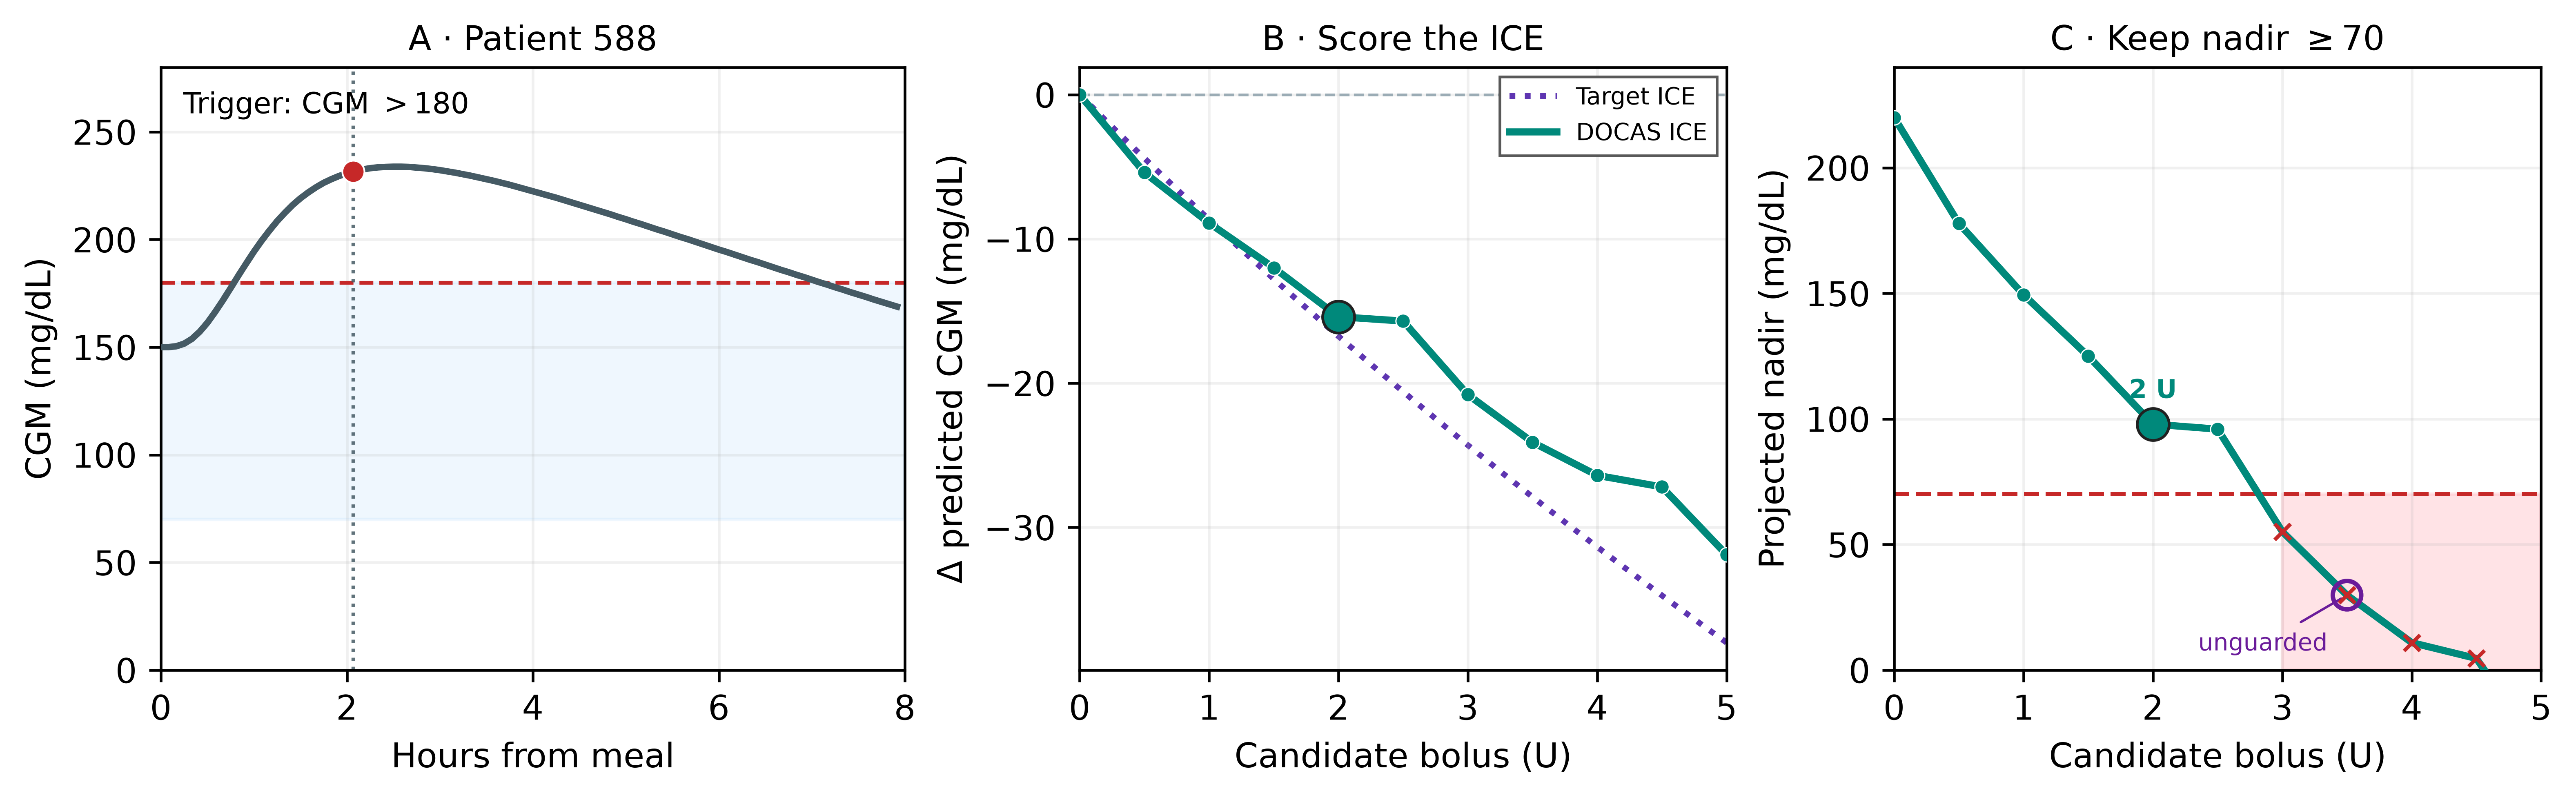
\includegraphics[width=\textwidth]{figures/safeguard_patient588.png}
  \caption{Hypoglycaemia-guard loop on OhioT1DM patient~588.
  \textbf{A:} hyperglycaemia trigger (CGM~$>180$~mg/dL, red dashed) at the
  decision time (vertical dotted).
  \textbf{B:} each candidate bolus scored on the ICE against the target
  DRC.
  \textbf{C:} projected worst-case nadir versus dose; crosses below $70$~mg/dL
  are inadmissible. Filled marker: guarded pick; open marker: unguarded pick on
  the same ICE.}
  \label{fig:safety}
\end{figure*}

Table~\ref{tab:unguarded} removes the guard on the same windows, twins, cost,
target, trigger, penalty, and search grid. The observational arm also moves
($1.09\to 1.32$~U, post-decision TIR $73.61\to 73.86\%$). DOCAS insulin rises from $2.23$ to
$2.91$~U; post-decision TIR is nearly unchanged ($76.01\to 75.76\%$) but TBR appears
($1.26\%$), all from patient~588 at start~$1962$
(Figure~\ref{fig:ohio-replay}: $3.5\to 6.5$~U, $13.89\%$ below range after the
first decision). That twin
sits at $1.30\times$ the prior modal~$S_I$, inside the $2\times$ margin; without
the margin the rejected dose looks safe (nadir $125$~mg/dL) even though the twin
drops below $70$~mg/dL. The guard corrects optimism of a 60-minute cost that has
not yet seen the nadir. Alignment does not by itself limit how much insulin is
given; a trajectory forecaster could penalise late hypoglycaemia directly.

\FloatBarrier
\begin{table}[pos=htbp,width=0.72\linewidth]
\centering
\caption{The same 11 OhioT1DM windows from 4 participants and the same CIB cost as Table~\ref{tab:replay}, but without the hypoglycaemia guard (no $70$~mg/dL floor, no $2\times$ margin), i.e.\ Prendin-faithful scoring. TIR, TBR, and TAR are post-decision. Mean~$\pm$~SD.}
\label{tab:unguarded}
\scriptsize
\begin{tabular}{lccc}
\toprule
Metric & No DSS & Baseline & DOCAS \\
\midrule
TBR (\%) & 0.00 $\pm$ 0.00 & 0.00 $\pm$ 0.00 & 1.26 $\pm$ 4.19 \\
TIR (\%) & 61.49 $\pm$ 34.22 & 73.86 $\pm$ 23.92 & 75.76 $\pm$ 23.12 \\
TAR (\%) & 38.51 $\pm$ 34.22 & 26.14 $\pm$ 23.92 & 22.98 $\pm$ 21.11 \\
Insulin (U) & 0.00 $\pm$ 0.00 & 1.32 $\pm$ 1.35 & 2.91 $\pm$ 2.77 \\
\bottomrule
\end{tabular}
\end{table}

\FloatBarrier

\section{Supplementary: a pump-settings target DRC}\label{app:clinical-tau}

The alignment follows whichever dose--response is supplied, so this appendix repeats it on a second curve taken from each participant's pump settings rather than from the UVa/Padova DRC used in the main study.
The last ablation row of Table~\ref{tab:ablation} replaces the UVa/Padova target
DRC with a pump-settings curve~\citep{walsh2011}:
\begin{equation}
  \tau_H(u;\,g) \;=\; -\,\frac{1800}{\mathrm{TDD}}\; u \; A(H)\;\frac{g}{G_0},
  \label{eq:pump-tau}
\end{equation}
where $1800/\mathrm{TDD}$ is the participant's correction factor (mg/dL per unit
at $G_0{=}220$~mg/dL; OhioT1DM median $34$, range $17$--$74$; AZT1D $51$,
$15$--$100$) and $A(H)$ is the insulin-action share by horizon~$H$
($t_p{=}75$~min, $t_d{=}300$~min; $A(30){=}0.075$, $A(60){=}0.236$). The product
is linear in dose and personal rather than cohort-wide. At $G_0$ a unit lowers
glucose by $2.69$ and $8.46$~mg/dL on average in OhioT1DM at 30 and 60~min
($3.87$ and $12.17$ in AZT1D). Against the UVa/Padova curve ($0.74$ and
$8.25$~mg/dL per unit) the two constructions nearly coincide at 60~min but
disagree at 30~min, where UVa/Padova puts more delay into early insulin action.

$\mathrm{TDD}$ is mean daily basal plus bolus. On AZT1D, basal rates above
5~U/h are excluded and $\mathrm{TDD}$ is clipped to $18$--$120$~U/day (correction
factor $100$--$15$~mg/dL per unit). Forecasting results are in
Table~\ref{tab:ablation}.

Table~\ref{tab:clinical-replay} repeats the ReplayBG protocol on the same eleven
windows with DOCAS retrained on Eq.~\ref{eq:pump-tau}. Twins, screens, baseline,
and UVa/Padova DOCAS are unchanged. Post-decision TIR rises to $75.88\%$
(vs.\ $73.61\%$ Baseline, $76.01\%$ UVa/Padova DOCAS) on $2.36$~U with zero TBR under the
same guard. The dosing gain is still there when the supplied curve is this pump-settings DRC.

\FloatBarrier
\begin{table}[pos=htbp,width=0.92\linewidth]
\centering
\caption{Same 11 OhioT1DM windows and hypoglycaemia guard as Table~\ref{tab:replay} (4 participants), with DOCAS retrained on each patient's pump-settings DRC. Study-DRC DOCAS columns are the main-text arm. TIR, TBR, and TAR are post-decision. Mean~$\pm$~SD.}
\label{tab:clinical-replay}
\scriptsize
\begin{tabular}{lcccc}
\toprule
Metric & No DSS & Baseline & DOCAS (study DRC) & DOCAS (pump-settings DRC) \\
\midrule
TBR (\%) & 0.00 $\pm$ 0.00 & 0.00 $\pm$ 0.00 & 0.00 $\pm$ 0.00 & 0.00 $\pm$ 0.00 \\
TIR (\%) & 61.49 $\pm$ 34.22 & 73.61 $\pm$ 23.83 & 76.01 $\pm$ 21.95 & 75.88 $\pm$ 21.91 \\
TAR (\%) & 38.51 $\pm$ 34.22 & 26.39 $\pm$ 23.83 & 23.99 $\pm$ 21.95 & 24.12 $\pm$ 21.91 \\
Insulin (U) & 0.00 $\pm$ 0.00 & 1.09 $\pm$ 1.41 & 2.23 $\pm$ 2.04 & 2.36 $\pm$ 2.58 \\
\bottomrule
\end{tabular}
\end{table}

\FloatBarrier

\bibliographystyle{model1-num-names}
\bibliography{references}

\end{document}
